\documentclass[a4paper,10.5pt]{article}
\usepackage{mathtools}
\usepackage{listings}
\usepackage{tikz-qtree}
\usepackage{dirtree}
\usepackage[utf8x]{inputenc}
\usepackage[font=small,format=plain,labelfont=bf,up,textfont=normal,up]{caption}
\usepackage[left=2.2cm,top=2cm,right=2.2cm,bottom=2cm,nohead,nofoot]{geometry}
\usepackage{wrapfig}
\usepackage{graphicx}
\usepackage{subcaption}

\setlength{\footskip}{25pt}
\usepackage{tikz}
\usepackage{amsmath,tikz}
\usetikzlibrary{shapes.geometric}
\usepackage{subcaption}
\usepackage{pgfplots}
\usepackage{filecontents}
\usepackage{algpseudocode}
\usepackage{algorithm}
\usepackage{subfig}
\usepackage{float}
\usepackage{graphicx}
\usepackage{marginnote}
\usepackage{pgfgantt}
\usepackage{pdflscape}
\usepackage{wrapfig}
\usepackage{tikz}

\usepackage{forest}
\usepackage{tikz-qtree}

\usepackage{listings}
\usepackage{color}
\usepackage{pgfplots}
\usepackage{filecontents}
\pgfdeclarelayer{background}
\usetikzlibrary{matrix}
\usetikzlibrary{shapes,arrows}

\definecolor{mygreen}{rgb}{0,0.6,0}
\definecolor{mygray}{rgb}{0.5,0.5,0.5}
\definecolor{mylightgray}{HTML}{F2F2F2}
\definecolor{mymauve}{rgb}{0.58,0,0.82}
\makeatletter
\newenvironment{customlegend}[1][]{%
    \begingroup
    % inits/clears the lists (which might be populated from previous
    % axes):
    \pgfplots@init@cleared@structures
    \pgfplotsset{#1}%
}{%
    % draws the legend:
    \pgfplots@createlegend
    \endgroup
}%

\def\addlegendimage{\pgfplots@addlegendimage}
\makeatother
\lstset{ language=C,
  backgroundcolor=\color{mylightgray},   % choose the background color; you must add \usepackage{color} or \usepackage{xcolor}
showstringspaces=false,
belowcaptionskip=0em,
    belowskip=-1em,
  basicstyle=\footnotesize,        % the size of the fonts that are used for the code
  breakatwhitespace=false,         % sets if automatic breaks should only happen at whitespace
  breaklines=true,                 % sets automatic line breaking
  captionpos=b,                    % sets the caption-position to bottom
  commentstyle=\color{mygreen},    % comment style
  deletekeywords={...},            % if you want to delete keywords from the given language
  escapeinside={\%*}{*)},          % if you want to add LaTeX within your code
  extendedchars=true,              % lets you use non-ASCII characters; for 8-bits encodings only, does not work with UTF-8
  frame=single,                    % adds a frame around the code
  keepspaces=true,                 % keeps spaces in text, useful for keeping indentation of code (possibly needs columns=flexible)
  keywordstyle=\color{blue},       % keyword style
  language=C,                 % the language of the code
  morekeywords={*,...},            % if you want to add more keywords to the set
  numbers=left,                    % where to put the line-numbers; possible values are (none, left, right)
  numbersep=5pt,                   % how far the line-numbers are from the code
  numberstyle=\tiny\color{mygray}, % the style that is used for the line-numbers
  rulecolor=\color{white},         % if not set, the frame-color may be changed on line-breaks within not-black text (e.g. comments (green here))
  showspaces=false,                % show spaces everywhere adding particular underscores; it overrides 'showstringspaces'
  showstringspaces=false,          % underline spaces within strings only
  showtabs=false,                  % show tabs within strings adding particular underscores
  stepnumber=0,                    % the step between two line-numbers. If it's 1, each line will be numbered
  stringstyle=\color{mymauve},     % string literal style
  tabsize=2,                       % sets default tabsize to 2 spaces
  title=\lstname                  % show the filename of files included with \lstinputlisting; also try caption instead of title
}

\renewcommand{\footnoterule}{%
  \kern -3pt
  \hrule width \textwidth height 0.5pt
  \kern 2pt
}
\tikzstyle{decision} = [diamond, draw, fill=white!20, 
    text width=6em, text badly centered, node distance=3cm, inner sep=1pt]
\tikzstyle{block} = [rectangle, draw, fill=white!20, 
    text width=5em, text centered, rounded corners, minimum height=3em]
\tikzstyle{line} = [draw, -latex']
\tikzset{
  treenode/.style = {align=center, inner sep=0pt, text centered,
    font=\sffamily},
 arn_n/.style = {treenode, circle, white,  font=\sffamily, draw=black,
    fill=black, text width=1.5em}
}
\usepackage{marginnote}
\usepackage{pgfgantt}
\usepackage{rotating}
\usepackage{pdflscape}
\usepackage{float}
\usepackage{tablefootnote}
\title{Random Number Generation Using Genetic Programming}
\author{{\small by}\\\\Philip Leonard\\ 200714801 \\\\\\\\ A Dissertation \\\\\\\\ {\large Submitted to} \\\\{\Large The University of Liverpool} \\\\\\{\normalsize  in partial fulfillment of the requirements for the degree of}\\\\{\Large BSc Computer Science}}

\tikzset{
    maxfitnessorgen /.style={
        /pgfplots/execute at end plot visualization={\draw [current plot style, dashed] (@auxnode.center) -- ($(@auxnode.center)!10cm!(@auxnode.east)$);}
    },
    maxfitnessorgen nodestyle/.style={
        pos=1, inner sep=0pt, sloped, alias=@auxnode
    }
}
\definecolor{lblue}{HTML}{33B5E5}
\definecolor{lgrey}{HTML}{7F8C8D}
\definecolor{lpurple}{HTML}{AA66CC}
\definecolor{lgreen}{HTML}{99CC00}
\definecolor{lorange}{HTML}{FFBB33}
\definecolor{lred}{HTML}{FF4444}
\definecolor{dblue}{HTML}{0099CC}
\definecolor{dpurple}{HTML}{9933CC}
\definecolor{dgreen}{HTML}{669900}
\definecolor{dorange}{HTML}{FF8800}
\definecolor{dred}{HTML}{CC0000}

\pgfplotscreateplotcyclelist{androidstyle}{
{dblue},
{lred},
{lorange},
{lgreen},
{lpurple},
{dorange},
{lgrey},
}

\pgfplotscreateplotcyclelist{androidstyle2}{
{lblue},
{lred},
}

\begin{filecontents}{data3.dat}
a b c
1	99.96729643	0.032703571
2	99.97726786	0.022732143
3	99.98027143	0.019728571
4	99.967075	0.032925
5	99.96595357	0.034046429
6	99.981325	0.018675
7	99.97520357	0.024796429
8	99.96810357	0.031896429
9	99.969	0.031
10	99.96637857	0.033621429
11	99.97191071	0.028089286
12	99.9644	0.0356
13	99.97497143	0.025028571
14	99.96993214	0.030067857
15	99.98225714	0.017742857
16	99.97026071	0.029739286
17	99.96808929	0.031910714
18	99.96448214	0.035517857
19	99.97425	0.02575
20	99.966675	0.033325


\end{filecontents}
\begin{filecontents}{data2.dat}
a b c d
1	0	99.97296071	0.027039286
2	0	99.96640357	0.033596429
3	0	99.96866429	0.031335714
4	0	99.96780714	0.032192857
5	0	99.97332143	0.026678571
6	0	99.97695	0.02305
7	0	99.98063929	0.019360714
8	0	99.97420714	0.025792857
9	0	99.96871429	0.031285714
10	0	99.97333214	0.026667857
11	0	99.96508571	0.034914286
12	0	99.96811786	0.031882143
13	0	99.96981429	0.030185714
14	0	99.967475	0.032525
15	0	99.97418929	0.025810714
16	0	99.98474643	0.015253571
17	0	99.96928214	0.030717857
18	0	99.97070357	0.029296429
19	0	99.97949643	0.020503571
20	0	99.97775	0.02225
21	0	99.96590714	0.034092857
22	0	99.96549643	0.034503571
23	0	99.96542857	0.034571429
24	0	99.96529643	0.034703571
25	0	99.97286071	0.027139286
26	0	99.97101786	0.028982143
27	0	99.96598929	0.034010714
28	0	99.974	0.026
29	0	99.97137143	0.028628571
30	0	99.97784286	0.022157143
31	0	99.96619643	0.033803571
32	0	99.97228929	0.027710714
33	0	99.96756071	0.032439286
34	0	99.96518929	0.034810714
35	0	99.96739643	0.032603571
36	0	99.965275	0.034725
37	0	99.97100714	0.028992857
38	0	99.96836786	0.031632143
39	0	99.97608571	0.023914286
40	0	99.96618571	0.033814286
41	0	99.96618929	0.033810714
42	0	99.96989286	0.030107143
43	0	99.96644286	0.033557143
44	0	99.96870357	0.031296429
45	0	99.97503214	0.024967857



\end{filecontents}

\begin{filecontents}{data.dat}
a b c d e f g h
0 0 0 0 0 27.99 3500 0
5.215	7	31.261002	15.094717  3500 27.99 3500 27.99
6.414	7	60.902	19.105244
9.022	7	90.228996	19.10527
9.135	7	120.320999	22.976607
10.721	7	151.761993	27.140421
12.149	7	184.912994	22.893248
17.468	7	218.873993	22.07391
17.556	7	254.303009	22.828935
17.629999	7	291.924011	23.645366
20.441999	7	330.677002	24.311918
21.146999	7	371.444	24.311918
22.165001	7	416.319	26.649654
22.271	7	464.31601	27.429894
23.767	7	518.906006	27.429894
24.483999	7	569.281982	27.739345
25.183001	7	621.880981	27.615823
25.775999	7	680.329041	27.250725
25.886	7	741.445007	27.840851
26.080999	7	802.234985	27.148943
26.709999	13	865.580994	27.182579
26.771999	13	932.15802	27.704818
26.959999	17.319771	1005.679993	27.321578
27.201	17.319771	1086.596069	27.71119
30.58	17.319771	1163.189087	27.940605
30.923	17.319771	1244.552002	27.921593
31.951	17.319771	1341.045044	27.610104
32.008999	17.319771	1435.526978	27.919134
32.949001	17.319771	1537.971924	27.182084
33.133999	17.319771	1640.754028	27.535916
34.431	17.319771	1749.439941	27.536886
34.773998	17.319771	1865.084961	27.378717
34.834	17.319771	1982.332031	27.650268
36.011002	17.319771	2103.302002	27.368844
37.271999	17.319771	2231.157959	27.906107
39.213001	17.319771	2362.587891	27.335561
39.627998	17.319771	2490.022949	27.86676
43.209999	17.319771	2629.313965	27.651825
43.470001	17.319771	2770.828857	27.431928
43.823002	17.319771	2920.779053	27.431928
44.563	17.319771	3071.5	27.431928
44.619999	17.319771	3227.51001	27.431928
45.324001	17.319771	3399.604004	27.99132
45.389	17.319771		
45.457001	17.319771		
47.953999	17.319868		
48.014999	17.319868		
48.799	17.319868		
48.855999	17.319868		
49.459	17.319868		
50.571999	17.319868		
51.292999	17.319868		
51.539001	17.319868		
52.023998	17.319868		
55.383999	17.319868		
56.009998	18.25359		
56.132	18.25359		
58.824001	18.25359		
59.063	18.25359		
59.686001	18.25359		
60.973999	18.25359		
61.970001	27.372338		
62.085999	27.372338		
67.675003	27.372341		
70.528	27.372341		
74.498001	27.372341		
75.097	27.373927		
75.814003	27.373927		
75.894997	27.374		
77.392998	27.374		
79.167	27.374		
81.098	27.374		
81.399002	27.374		
83.089996	27.374		
83.204002	27.374		
83.309998	27.374		
84.041	27.374		
87.849998	27.417114		
89.578003	27.069083		
89.976997	27.493499		
90.785004	27.493317		
90.864998	27.493317		
91.540001	27.493313		
91.904999	27.493313		
93.735001	27.493693		
96.262001	27.535502		
96.332001	27.535502		
96.695	27.535502		
100.563004	27.535502		
100.886002	27.535502		
101.322998	27.535502		
102.389	27.535097		
103.074997	27.535227		
106.283997	27.084255		
109.688004	27.360055		
110.069	27.360055		
110.404999	27.360055		
111.401001	27.360055		
111.802002	27.360055		
112.954002	27.360055		
115.510002	27.360055		
116.295998	27.360055		
116.440002	27.360055		
119.925003	27.575504		
120.720001	27.738019		
124.549004	27.928335		
124.841003	27.928335		
125.055	27.928335		
125.203003	27.928335		
125.568001	27.928335		
125.625	27.928335		
130.149002	27.981491		
131.914993	27.919683		
134.604996	27.919683		
135.192001	27.844016		
135.315002	27.844016		
135.496002	27.844016		
139.322998	27.844016		
139.427994	27.844016		
145.748993	27.844016		
145.895004	27.844016		
151.283997	27.844016		
156.259995	27.844016		
160.330002	27.945811		
160.682007	27.945811		
160.860001	27.945811		
164.397995	27.940644		
164.464005	27.940644		
164.623001	27.940644		
164.938004	27.940644		
165.106003	27.940644		
165.792999	27.940644		
170.348007	27.945171		
171.639008	27.945171		
178.516998	27.91403		
191.606003	27.91403		
191.785004	27.91403		
196.289993	27.91403		
199.141998	27.930084		
202.384003	27.930084		
202.826004	27.930084		
202.919006	27.930084		
205.296005	27.930084		
212.990997	27.930084		
217.656006	27.930084		
219.501007	27.930084		
233.339005	27.930084		
249.112	27.930084		
250.738007	27.930084		
250.794998	27.930084		
255.720001	27.930084		
263	27.930084		
263.34201	27.930084		
263.614014	27.930084		
273.286987	27.930084		
277.126007	27.930084		
277.203003	27.930084		
277.605011	27.933068		
283.580994	27.933068		
296.061005	27.933068		
306.69101	27.933068		
310.354004	27.933068		
318.44101	27.933068		
320.255005	27.933068		
321.157013	27.933068		
321.700012	27.933068		
321.941986	27.933068		
322.078003	27.934698		
322.912994	27.934698		
332.03299	27.934698		
338.834015	27.934698		
338.903015	27.934698		
340.708008	27.934698		
340.877014	27.950286		
354.384003	27.950286		
354.459991	27.950286		
362.644012	27.950286		
371.123993	27.950286		
371.375	27.950286		
379.88501	27.950286		
384.619995	27.950286		
394.36499	27.986559		
407.100006	27.986559		
407.940002	27.986559		
412.709015	27.986559		
420.131989	27.986559		
432.546997	27.986559		
432.673004	27.986559		
433.075989	27.986559		
440.769989	27.986559		
440.901001	27.986559		
456.673004	27.986559		
458.161011	27.986559		
467.721985	27.986559		
468.839996	27.986559		
498.631012	27.986559		
498.877991	27.986559		
507.074005	27.986559		
529.937988	27.986559		
543.669006	27.986559		
550.661987	27.986559		
562.653015	27.986559		
564.314026	27.986559		
570.039978	27.986559		
586.422974	27.986559		
604.356018	27.986559		
622.836975	27.988391		
622.911011	27.988391		
624.599976	27.99272		
\end{filecontents}

\begin{filecontents}{data5.dat}
a b c d e f g h
31.261002	0.918296	1.584962	2.251609	2.584962	2.584962	2.584962	2.584962
60.902	0.918357	1.825119	2.688667	3.084871	3.418306	3.584962	3.584962
90.228996	0.918357	1.825022	2.688728	3.084932	3.418306	3.584962	3.584962
120.320999	1	2	2.918255	3.636839	4.251588	4.584962	4.584962
151.761993	0.995418	1.98746	2.973344	3.927226	4.851823	5.755796	6.649353
184.912994	1	2	2.918255	3.636778	4.168291	4.584962	4.584962
218.873993	0.989872	1.926645	2.855979	3.572708	3.95289	4.247124	4.528692
254.303009	1	2	3	3.688715	4.136911	4.418346	4.584962
291.924011	0.899977	1.772705	2.622339	3.461632	4.249074	4.987058	5.652581
330.677002	0.99105	1.982023	2.972905	3.8774	4.593346	4.892028	5.003166
371.444	0.99105	1.982023	2.972905	3.8774	4.593346	4.892028	5.003166
416.319	0.997097	1.960847	2.919041	3.867582	4.795595	5.686447	6.423046
464.31601	0.99982	1.999525	2.991977	3.977944	4.928832	5.871955	6.659842
518.906006	0.99982	1.999525	2.991977	3.977944	4.928832	5.871955	6.659842
569.281982	0.999958	1.998028	2.995647	3.990225	4.963232	5.922526	6.869728
621.880981	0.999997	1.999654	2.998858	3.981387	4.956904	5.918982	6.760041
680.329041	0.999225	1.984675	2.969465	3.943999	4.905592	5.837535	6.610235
741.445007	0.999998	1.997595	2.995141	3.984531	4.973184	5.958659	6.931743
802.234985	0.999219	1.998432	2.997635	3.956649	4.892231	5.753892	6.550884
865.580994	0.99379	1.98629	2.965202	3.935263	4.881293	5.817699	6.603042
932.15802	1	1.999048	2.998031	3.975514	4.948896	5.918268	6.86506
1005.679993	0.9985	1.9869	2.973449	3.951665	4.90806	5.831784	6.671221
1086.596069	0.996668	1.993326	2.98953	3.984869	4.961284	5.922109	6.863404
1163.189087	0.999979	1.999955	2.999081	3.997297	4.993761	5.984752	6.96578
1244.552002	0.999458	1.998808	2.997637	3.995775	4.990111	5.981329	6.958477
1341.045044	0.999974	1.999766	2.998579	3.977825	4.944784	5.894935	6.794242
1435.526978	0.999978	1.999691	2.999168	3.997787	4.99101	5.976959	6.954541
1537.971924	0.999831	1.985222	2.968295	3.931844	4.88704	5.792655	6.617197
1640.754028	0.998731	1.997433	2.980887	3.957664	4.925454	5.886266	6.789481
1749.439941	0.998746	1.997465	2.980933	3.957729	4.925612	5.886541	6.78986
1865.084961	0.99988	1.999744	2.964439	3.927537	4.889153	5.836006	6.761958
1982.332031	0.999378	1.99647	2.991983	3.977996	4.960209	5.924135	6.800097
2103.302002	0.999519	1.986298	2.968352	3.942571	4.905243	5.848596	6.718265
2231.157959	0.999994	1.999962	2.999911	3.999756	4.999499	5.998194	6.908793
2362.587891	0.988262	1.976471	2.964522	3.946169	4.910449	5.832094	6.717593
2490.022949	0.999999	1.999882	2.999758	3.996867	4.992245	5.985511	6.892499
2629.313965	0.999996	1.999639	2.98917	3.978483	4.955352	5.929982	6.799202
2770.828857	0.982384	1.96456	2.946135	3.924148	4.900505	5.8739	6.840296
2920.779053	0.982384	1.96456	2.946135	3.924148	4.900505	5.8739	6.840296
3071.5	0.982384	1.96456	2.946135	3.924148	4.900505	5.8739	6.840296
3227.51001	0.982384	1.96456	2.946135	3.924148	4.900505	5.8739	6.840296
3399.604004	1	1.999998	2.999884	3.999732	4.999012	5.997608	6.995085


\end{filecontents}

\begin{filecontents}{data4.dat}
a b c d e f g h
5.215	1	1	1	1	1	1	1	
6.414	1	1	1	1	1	1	1	
9.022	1	1	1	1	1	1	1	
9.135	1	1	1	1	1	1	1	
10.721	1	1	1	1	1	1	1	
12.149	1	1	1	1	1	1	1	
17.468	1	1	1	1	1	1	1	
17.556	1	1	1	1	1	1	1	
17.629999	1	1	1	1	1	1	1	
20.441999	1	1	1	1	1	1	1	
21.146999	1	1	1	1	1	1	1	
22.165001	1	1	1	1	1	1	1	
22.271	1	1	1	1	1	1	1	
23.767	1	1	1	1	1	1	1	
24.483999	1	1	1	1	1	1	1	
25.183001	1	1	1	1	1	1	1	
25.775999	1	1	1	1	1	1	1	
25.886	1	1	1	1	1	1	1	
26.080999	1	1	1	1	1	1	1	
26.709999	1	2	2	2	2	2	2	
26.771999	1	2	2	2	2	2	2	
26.959999	1	1.811157	2.499908	3	3.001989	3.002917	3.0038	
27.201	1	1.811157	2.499908	3	3.001989	3.002917	3.0038	
30.58	1	1.811157	2.499908	3	3.001989	3.002917	3.0038	
30.923	1	1.811157	2.499908	3	3.001989	3.002917	3.0038	
31.951	1	1.811157	2.499908	3	3.001989	3.002917	3.0038	
32.008999	1	1.811157	2.499908	3	3.001989	3.002917	3.0038	
32.949001	1	1.811157	2.499908	3	3.001989	3.002917	3.0038	
33.133999	1	1.811157	2.499908	3	3.001989	3.002917	3.0038	
34.431	1	1.811157	2.499908	3	3.001989	3.002917	3.0038	
34.773998	1	1.811157	2.499908	3	3.001989	3.002917	3.0038	
34.834	1	1.811157	2.499908	3	3.001989	3.002917	3.0038	
36.011002	1	1.811157	2.499908	3	3.001989	3.002917	3.0038	
37.271999	1	1.811157	2.499908	3	3.001989	3.002917	3.0038	
39.213001	1	1.811157	2.499908	3	3.001989	3.002917	3.0038	
39.627998	1	1.811157	2.499908	3	3.001989	3.002917	3.0038	
43.209999	1	1.811157	2.499908	3	3.001989	3.002917	3.0038	
43.470001	1	1.811157	2.499908	3	3.001989	3.002917	3.0038	
43.823002	1	1.811157	2.499908	3	3.001989	3.002917	3.0038	
44.563	1	1.811157	2.499908	3	3.001989	3.002917	3.0038	
44.619999	1	1.811157	2.499908	3	3.001989	3.002917	3.0038	
45.324001	1	1.811157	2.499908	3	3.001989	3.002917	3.0038	
45.389	1	1.811157	2.499908	3	3.001989	3.002917	3.0038	
45.457001	1	1.811157	2.499908	3	3.001989	3.002917	3.0038	
47.953999	1	1.811254	2.499908	3	3.001989	3.002917	3.0038	
48.014999	1	1.811254	2.499908	3	3.001989	3.002917	3.0038	
48.799	1	1.811254	2.499908	3	3.001989	3.002917	3.0038	
48.855999	1	1.811254	2.499908	3	3.001989	3.002917	3.0038	
49.459	1	1.811254	2.499908	3	3.001989	3.002917	3.0038	
50.571999	1	1.811254	2.499908	3	3.001989	3.002917	3.0038	
51.292999	1	1.811254	2.499908	3	3.001989	3.002917	3.0038	
51.539001	1	1.811254	2.499908	3	3.001989	3.002917	3.0038	
52.023998	1	1.811254	2.499908	3	3.001989	3.002917	3.0038	
55.383999	1	1.811254	2.499908	3	3.001989	3.002917	3.0038	
56.009998	0.815149	1.504904	2.160932	2.754822	3.27247	3.684988	4.060326	
56.132	0.815149	1.504904	2.160932	2.754822	3.27247	3.684988	4.060326	
58.824001	0.815149	1.504904	2.160932	2.754822	3.27247	3.684988	4.060326	
59.063	0.815149	1.504904	2.160932	2.754822	3.27247	3.684988	4.060326	
59.686001	0.815149	1.504904	2.160932	2.754822	3.27247	3.684988	4.060326	
60.973999	0.815149	1.504904	2.160932	2.754822	3.27247	3.684988	4.060326	
61.970001	1	1.999955	2.994917	3.951705	4.9008	5.813808	6.711153	
62.085999	1	1.999955	2.994917	3.951705	4.9008	5.813808	6.711153	
67.675003	1	1.999954	2.994927	3.951754	4.900841	5.813771	6.711095	
70.528	1	1.999954	2.994927	3.951754	4.900841	5.813771	6.711095	
74.498001	1	1.999954	2.994927	3.951754	4.900841	5.813771	6.711095	
75.097	1	1.999961	2.994984	3.951934	4.901186	5.814215	6.711648	
75.814003	1	1.999961	2.994984	3.951934	4.901186	5.814215	6.711648	
75.894997	1	1.999959	2.99497	3.951968	4.901189	5.814225	6.711688	
77.392998	1	1.999959	2.99497	3.951968	4.901189	5.814225	6.711688	
79.167	1	1.999959	2.99497	3.951968	4.901189	5.814225	6.711688	
81.098	1	1.999959	2.99497	3.951968	4.901189	5.814225	6.711688	
81.399002	1	1.999959	2.99497	3.951968	4.901189	5.814225	6.711688	
83.089996	1	1.999959	2.99497	3.951968	4.901189	5.814225	6.711688	
83.204002	1	1.999959	2.99497	3.951968	4.901189	5.814225	6.711688	
83.309998	1	1.999959	2.99497	3.951968	4.901189	5.814225	6.711688	
84.041	1	1.999959	2.99497	3.951968	4.901189	5.814225	6.711688	
87.849998	0.999999	1.999896	2.995306	3.956455	4.910328	5.827664	6.727467	
89.578003	0.999772	1.995241	2.98641	3.92295	4.847606	5.726704	6.590399	
89.976997	0.999988	1.998661	2.996753	3.976163	4.926487	5.845864	6.749582	
90.785004	0.999989	1.998647	2.99672	3.976076	4.926419	5.845845	6.749622	
90.864998	0.999989	1.998647	2.99672	3.976076	4.926419	5.845845	6.749622	
91.540001	0.999988	1.998654	2.99673	3.976103	4.926441	5.845815	6.749583	
91.904999	0.999988	1.998654	2.99673	3.976103	4.926441	5.845815	6.749583	
93.735001	0.999989	1.998662	2.996755	3.97616	4.926514	5.845946	6.749667	
96.262001	0.999961	1.997809	2.994711	3.977243	4.936738	5.862638	6.766402	
96.332001	0.999961	1.997809	2.994711	3.977243	4.936738	5.862638	6.766402	
96.695	0.999961	1.997809	2.994711	3.977243	4.936738	5.862638	6.766402	
100.563004	0.999961	1.997809	2.994711	3.977243	4.936738	5.862638	6.766402	
100.886002	0.999961	1.997809	2.994711	3.977243	4.936738	5.862638	6.766402	
101.322998	0.999961	1.997809	2.994711	3.977243	4.936738	5.862638	6.766402	
102.389	0.999959	1.997833	2.994745	3.977299	4.936746	5.862463	6.76605	
103.074997	0.999958	1.997822	2.994721	3.977265	4.936733	5.862523	6.766205	
106.283997	0.999988	1.997531	2.986296	3.928189	4.839835	5.730131	6.602285	
109.688004	0.999992	1.999954	2.995387	3.951396	4.899753	5.809806	6.703767	
110.069	0.999992	1.999954	2.995387	3.951396	4.899753	5.809806	6.703767	
110.404999	0.999992	1.999954	2.995387	3.951396	4.899753	5.809806	6.703767	
111.401001	0.999992	1.999954	2.995387	3.951396	4.899753	5.809806	6.703767	
111.802002	0.999992	1.999954	2.995387	3.951396	4.899753	5.809806	6.703767	
112.954002	0.999992	1.999954	2.995387	3.951396	4.899753	5.809806	6.703767	
115.510002	0.999992	1.999954	2.995387	3.951396	4.899753	5.809806	6.703767	
116.295998	0.999992	1.999954	2.995387	3.951396	4.899753	5.809806	6.703767	
116.440002	0.999992	1.999954	2.995387	3.951396	4.899753	5.809806	6.703767	
119.925003	0.999964	1.996447	2.98915	3.963594	4.927029	5.878133	6.821187	
120.720001	0.999973	1.999244	2.998345	3.987358	4.963786	5.920783	6.868531	
124.549004	1	1.999854	2.999504	3.993606	4.987456	5.979388	6.968528	
124.841003	1	1.999854	2.999504	3.993606	4.987456	5.979388	6.968528	
125.055	1	1.999854	2.999504	3.993606	4.987456	5.979388	6.968528	
125.203003	1	1.999854	2.999504	3.993606	4.987456	5.979388	6.968528	
125.568001	1	1.999854	2.999504	3.993606	4.987456	5.979388	6.968528	
125.625	1	1.999854	2.999504	3.993606	4.987456	5.979388	6.968528	
130.149002	0.999999	1.999998	2.999992	3.998883	4.997475	5.99485	6.990294	
131.914993	0.99994	1.999872	2.999543	3.993928	4.987985	5.976484	6.96193	
134.604996	0.99994	1.999872	2.999543	3.993928	4.987985	5.976484	6.96193	
135.192001	0.99995	1.999693	2.998758	3.987401	4.973052	5.953156	6.932007	
135.315002	0.99995	1.999693	2.998758	3.987401	4.973052	5.953156	6.932007	
135.496002	0.99995	1.999693	2.998758	3.987401	4.973052	5.953156	6.932007	
139.322998	0.99995	1.999693	2.998758	3.987401	4.973052	5.953156	6.932007	
139.427994	0.99995	1.999693	2.998758	3.987401	4.973052	5.953156	6.932007	
145.748993	0.99995	1.999693	2.998758	3.987401	4.973052	5.953156	6.932007	
145.895004	0.99995	1.999693	2.998758	3.987401	4.973052	5.953156	6.932007	
151.283997	0.99995	1.999693	2.998758	3.987401	4.973052	5.953156	6.932007	
156.259995	0.99995	1.999693	2.998758	3.987401	4.973052	5.953156	6.932007	
160.330002	0.999998	1.999947	2.999626	3.995866	4.991266	5.984053	6.975055	
160.682007	0.999998	1.999947	2.999626	3.995866	4.991266	5.984053	6.975055	
160.860001	0.999998	1.999947	2.999626	3.995866	4.991266	5.984053	6.975055	
164.397995	0.999993	1.999971	2.999763	3.996209	4.991205	5.982234	6.971268	
164.464005	0.999993	1.999971	2.999763	3.996209	4.991205	5.982234	6.971268	
164.623001	0.999993	1.999971	2.999763	3.996209	4.991205	5.982234	6.971268	
164.938004	0.999993	1.999971	2.999763	3.996209	4.991205	5.982234	6.971268	
165.106003	0.999993	1.999971	2.999763	3.996209	4.991205	5.982234	6.971268	
165.792999	0.999993	1.999971	2.999763	3.996209	4.991205	5.982234	6.971268	
170.348007	0.999939	1.999879	2.999447	3.996562	4.991939	5.983527	6.973878	
171.639008	0.999939	1.999879	2.999447	3.996562	4.991939	5.983527	6.973878	
178.516998	0.999997	1.999988	2.999908	3.995031	4.98753	5.973592	6.957984	
191.606003	0.999997	1.999988	2.999908	3.995031	4.98753	5.973592	6.957984	
191.785004	0.999997	1.999988	2.999908	3.995031	4.98753	5.973592	6.957984	
196.289993	0.999997	1.999988	2.999908	3.995031	4.98753	5.973592	6.957984	
199.141998	0.999067	1.997603	2.995921	3.994082	4.989692	5.982666	6.971053	
202.384003	0.999067	1.997603	2.995921	3.994082	4.989692	5.982666	6.971053	
202.826004	0.999067	1.997603	2.995921	3.994082	4.989692	5.982666	6.971053	
202.919006	0.999067	1.997603	2.995921	3.994082	4.989692	5.982666	6.971053	
205.296005	0.999067	1.997603	2.995921	3.994082	4.989692	5.982666	6.971053	
212.990997	0.999067	1.997603	2.995921	3.994082	4.989692	5.982666	6.971053	
217.656006	0.999067	1.997603	2.995921	3.994082	4.989692	5.982666	6.971053	
219.501007	0.999067	1.997603	2.995921	3.994082	4.989692	5.982666	6.971053	
233.339005	0.999067	1.997603	2.995921	3.994082	4.989692	5.982666	6.971053	
249.112	0.999067	1.997603	2.995921	3.994082	4.989692	5.982666	6.971053	
250.738007	0.999067	1.997603	2.995921	3.994082	4.989692	5.982666	6.971053	
250.794998	0.999067	1.997603	2.995921	3.994082	4.989692	5.982666	6.971053	
255.720001	0.999067	1.997603	2.995921	3.994082	4.989692	5.982666	6.971053	
263	0.999067	1.997603	2.995921	3.994082	4.989692	5.982666	6.971053	
263.34201	0.999067	1.997603	2.995921	3.994082	4.989692	5.982666	6.971053	
263.614014	0.999067	1.997603	2.995921	3.994082	4.989692	5.982666	6.971053	
273.286987	0.999067	1.997603	2.995921	3.994082	4.989692	5.982666	6.971053	
277.126007	0.999067	1.997603	2.995921	3.994082	4.989692	5.982666	6.971053	
277.203003	0.999067	1.997603	2.995921	3.994082	4.989692	5.982666	6.971053	
277.605011	0.99951	1.998133	2.996415	3.994471	4.990036	5.982791	6.971712	
283.580994	0.99951	1.998133	2.996415	3.994471	4.990036	5.982791	6.971712	
296.061005	0.99951	1.998133	2.996415	3.994471	4.990036	5.982791	6.971712	
306.69101	0.99951	1.998133	2.996415	3.994471	4.990036	5.982791	6.971712	
310.354004	0.99951	1.998133	2.996415	3.994471	4.990036	5.982791	6.971712	
318.44101	0.99951	1.998133	2.996415	3.994471	4.990036	5.982791	6.971712	
320.255005	0.99951	1.998133	2.996415	3.994471	4.990036	5.982791	6.971712	
321.157013	0.99951	1.998133	2.996415	3.994471	4.990036	5.982791	6.971712	
321.700012	0.99951	1.998133	2.996415	3.994471	4.990036	5.982791	6.971712	
321.941986	0.99951	1.998133	2.996415	3.994471	4.990036	5.982791	6.971712	
322.078003	0.999555	1.998207	2.996509	3.994597	4.990275	5.983195	6.972361	
322.912994	0.999555	1.998207	2.996509	3.994597	4.990275	5.983195	6.972361	
332.03299	0.999555	1.998207	2.996509	3.994597	4.990275	5.983195	6.972361	
338.834015	0.999555	1.998207	2.996509	3.994597	4.990275	5.983195	6.972361	
338.903015	0.999555	1.998207	2.996509	3.994597	4.990275	5.983195	6.972361	
340.708008	0.999555	1.998207	2.996509	3.994597	4.990275	5.983195	6.972361	
340.877014	0.999947	1.998967	2.997853	3.996491	4.993289	5.9869	6.976839	
354.384003	0.999947	1.998967	2.997853	3.996491	4.993289	5.9869	6.976839	
354.459991	0.999947	1.998967	2.997853	3.996491	4.993289	5.9869	6.976839	
362.644012	0.999947	1.998967	2.997853	3.996491	4.993289	5.9869	6.976839	
371.123993	0.999947	1.998967	2.997853	3.996491	4.993289	5.9869	6.976839	
371.375	0.999947	1.998967	2.997853	3.996491	4.993289	5.9869	6.976839	
379.88501	0.999947	1.998967	2.997853	3.996491	4.993289	5.9869	6.976839	
384.619995	0.999947	1.998967	2.997853	3.996491	4.993289	5.9869	6.976839	
394.36499	0.99999	1.999885	2.999702	3.999402	4.998358	5.996487	6.992735	
407.100006	0.99999	1.999885	2.999702	3.999402	4.998358	5.996487	6.992735	
407.940002	0.99999	1.999885	2.999702	3.999402	4.998358	5.996487	6.992735	
412.709015	0.99999	1.999885	2.999702	3.999402	4.998358	5.996487	6.992735	
420.131989	0.99999	1.999885	2.999702	3.999402	4.998358	5.996487	6.992735	
432.546997	0.99999	1.999885	2.999702	3.999402	4.998358	5.996487	6.992735	
432.673004	0.99999	1.999885	2.999702	3.999402	4.998358	5.996487	6.992735	
433.075989	0.99999	1.999885	2.999702	3.999402	4.998358	5.996487	6.992735	
440.769989	0.99999	1.999885	2.999702	3.999402	4.998358	5.996487	6.992735	
440.901001	0.99999	1.999885	2.999702	3.999402	4.998358	5.996487	6.992735	
456.673004	0.99999	1.999885	2.999702	3.999402	4.998358	5.996487	6.992735	
458.161011	0.99999	1.999885	2.999702	3.999402	4.998358	5.996487	6.992735	
467.721985	0.99999	1.999885	2.999702	3.999402	4.998358	5.996487	6.992735	
468.839996	0.99999	1.999885	2.999702	3.999402	4.998358	5.996487	6.992735	
498.631012	0.99999	1.999885	2.999702	3.999402	4.998358	5.996487	6.992735	
498.877991	0.99999	1.999885	2.999702	3.999402	4.998358	5.996487	6.992735	
507.074005	0.99999	1.999885	2.999702	3.999402	4.998358	5.996487	6.992735	
529.937988	0.99999	1.999885	2.999702	3.999402	4.998358	5.996487	6.992735	
543.669006	0.99999	1.999885	2.999702	3.999402	4.998358	5.996487	6.992735	
550.661987	0.99999	1.999885	2.999702	3.999402	4.998358	5.996487	6.992735	
562.653015	0.99999	1.999885	2.999702	3.999402	4.998358	5.996487	6.992735	
564.314026	0.99999	1.999885	2.999702	3.999402	4.998358	5.996487	6.992735	
570.039978	0.99999	1.999885	2.999702	3.999402	4.998358	5.996487	6.992735	
586.422974	0.99999	1.999885	2.999702	3.999402	4.998358	5.996487	6.992735	
604.356018	0.99999	1.999885	2.999702	3.999402	4.998358	5.996487	6.992735	
622.836975	0.999976	1.999949	2.999804	3.999331	4.998732	5.996929	6.99367	
622.911011	0.999976	1.999949	2.999804	3.999331	4.998732	5.996929	6.99367	
624.599976	0.999975	1.999923	2.999861	3.999666	4.999131	5.998094	6.99607	


\end{filecontents}

\begin{filecontents}{sngpreduced.dat}
a b
10 0
20 60
40 60
60 70
80 80
100 88
\end{filecontents}

\begin{filecontents}{gpreduced.dat}
a b
50 0
100 40
200 40
300 20
400 40
500 40
\end{filecontents}

\begin{filecontents}{gpreducedrun.dat}
a b
0 0
50 647.3
100 941.2
200 845.8
300 1716.1
400 2484.1
500 4111.6
\end{filecontents}

\begin{filecontents}{sngpreducedrun.dat}
a b
0 0
10 291.7
20 423.3
40 599.3
60 851.6
80 868.8
100 606.9
\end{filecontents}



\begin{filecontents}{cvsmyrand.dat}
a b c
10 0.000000 0.000000
100 0.000000 0.000000
1000 0.002000 0.000000
10000 0.026000 0.001000
100000 0.235000 0.004000	
1000000 2.400000 0.044000	 		
10000000 24.085001 0.477000
100000000 236.805008 4.573000
\end{filecontents}

\begin{filecontents}{cvsmyrandc.dat}
a b
10 0.000000
100 0.000000
1000 0.000000
10000 0.001000
100000 0.004000	
1000000 0.044000	 		
10000000 0.477000
100000000 4.573000
1000000000 46.348999
10000000000 463.489990
\end{filecontents}

\begin{filecontents}{rand_runtime.dat}
a b c
10 0.010000 0.000000
100 0.016000 0.000000	
1000 0.023000 0.000000
10000 0.030000 0.001000	
100000 0.037000 0.001000	
1000000 0.043000 0.001000	
10000000 0.054000 0.001000
\end{filecontents}


\begin{document}
\begin{titlepage}
\maketitle
\end{titlepage}

\tableofcontents
\newpage
\listoffigures
\listoftables
\newpage
\section{Abstract}

This is the final report for the project; `Random Number Generation Using Genetic Programming' by Philip Leonard, supervised by Dr David Jackson (primary supervisor) and Professor Paul Dunne (secondary supervisor). This document covers all aspects of the project from the introduction and background, to the design, implementation and analysis of the project in order to give the reader an understanding of how I implemented the project and what things I found when evaluating the project.

This report demonstrates that using methods described by Koza in \cite{kozarng}, it is possible to genetically breed Random Number Generators (RNG) that produce sequences of pseudo random bits with near maximal entropy. All of the steps for designing and implementing the Genetic Programming (GP) approach are covered in detail. The results I obtained for the GP approach are similar to those produced by Koza. This allowed me to then make fair comparisons to the other methods of producing RNGs.

This report more importantly shows that it is possible to produce better results using the Single Node Genetic Programming (SNGP) methodology described by Jackson in \cite{jacksonsngp}. Using the SNGP paradigm, I was able to achieve results showing that it possible to obtain smaller and higher entropy RNGs (on average) six times quicker and at twice the rate of Koza's standard GP implementation manages to achieve. The stages of designing and implementing the SNGP approach, like the GP approach, are covered in detail in this report.

As well as this, this report also demonstrates that the Random Number Generators Produced genetically by these methods also produce sequences of random bits with higher entropy than other widely used RNGs. It not only outperforms the C programming Linear Congruential Generator (LCG) algorithm implemented in the $rand()$ function, but can also perform better than a Hardware/``True" Random Number Generator that creates random bit sequences from observed atmospheric noise.

This report also shows how a RNG produced by these evolutionary means might be implemented for use in the C programming language, by showing a pragmatic approach for developers to achieve higher entropy random numbers for use in their applications and software. I also show however that this comes at the cost of increased computation time compared to the C $rand()$ function.

At the end of the document I also discuss some further research that can be carried out in order to find ways of further improving the results I obtained by modifying the GP and SNGP implementations. I also discuss the learning process through this project and explaining the new skills that I have acquired. I go onto discuss how this project conformed to the British Computer Society: Chartered Institute for IT's code of conduct and code of practice (where it is applicable).

All of the code for the implemented software can be found in the appendix of this report and on the CD provided. As well as this, all of the pdf documents produced for this project and the \LaTeX\ files used to create them can be found there, as well as all of the test data used in evaluating all of the approaches.
\newline

\noindent \textbf{Keywords:} Genetic Algorithm (GA), Genetic Programming/Program (GP), Pseudo Random Number Generator (PRNG), Random Number Generator (RNG), True Random Number Generator (TRNG), Entropy, Single Node Genetic Programming/Program (SNGP), Crossover, Mutation, Fitness Proportionate Reproduction (FPR), Linear Congruential Generator (LCG).\newline

\noindent \textbf{Word Count:} 14954 words\footnote{Words counted using \emph{TexCount} web service (v3.0.0.24) : http://app.uio.no/ifi/texcount/online.php}. Not including words in contents, appendix, bibliography, diagrams, equations, headings or code listings.
\newpage

\newpage
\section{Introduction}
%Whats a RNG?
Random Number Generators have many computational, scientific and societal applications. They are essential in; gambling, lottery draws, cryptography, statistical sampling, Monte Carlo simulations, randomized algorithms, password generation and other applications where an unpredictable result is desired. Randomness can be interpreted in more than one way and has no strict mathematical definition. There are a series of tests that can be run on a set of data in order to evaluate some conception of randomness. These include the gap test, frequency test, runs test and information entropy test amongst others described in the NIST\footnote{National Institute of Standards and Technology} ``\emph{Test Suite for Random and Pseudorandom Number Generators for Cryptographic Applications}" \cite{nist}. Whilst there isn't a way to prove randomness, these statistical tests are a good way of analysing randomness in the eyes of the user and for their practical application. In this project, randomness is tested using the Shannon Entropy equation \cite[p.2]{kozarng}, which is a measure of the unpredictability/uncertainty in a random variable.
A Pseudo Random Number Generator (PRNG) is a program/algorithm which generates numbers that possess the characteristics of a ``truly" random number. These programs typically employ seed values (an example being the number of nanoseconds since the Unix epoch\footnote{00:00:00 (UTC), Thursday, 1 January 1970}), or they use a sequence of consecutive numbers as an input. Mathematical operators are applied to this input in order to fabricate a ``random" number or bit sequence. This differs from true random number generators which typically use a piece of hardware to measure an unpredictable environmental occurrence such as radiation, measured by a Geiger Counter. 

%What is Genetic Programming - EXPAND ON THIS
The Genetic Programming paradigm is an evolutionary method of solving problems, where the implementer can define a task where solutions can be randomly generated and tested by some fitness function. The population can then be evolved based on their fitness in order to search through the problem space to find solutions which meet the fitness requirements of the implementer. 

%Aim of the Project
Evolving Random Number Generators is therefore an applicable problem instance for Genetic Programming, as there is no deterministic way of producing a RNG with high entropy.  The aim of the project is to assess two Genetic Programming methodologies in order to determine which is best suited for genetically breeding RNGs. The method described by Koza in \cite{kozarng} was followed in order to implement the idea of evolving a random number generator in the widely known traditional Genetic Programming methodology. The next step was to implement the same idea using the Single Node Genetic Programming Methodology described by Jackson in \cite{jacksonsngp}. The effectiveness of both where then compared by gathering data from both implementations and conducting some cross examination to determine the victor. In order to determine the effectiveness of the Random Number Generators as a real world solution, entropy data was gathered from pre-existing and widely used RNGs. These were namely the C rand function, which is a PRNG that makes use of a Linear Congruential Generator algorithm in order to produce random numbers, and a ``True" Random Number Generator was also evaluated in order to compare the effectiveness of the genetically produced RNGs against a non-deterministic source of random data. 

%Challanges of the project?
Attempting to match Koza's implementation was a one of the major challenges of the project. Koza doesn't give many details of how he implemented the Genetic Program. Instead he gives a theoretical overview of the operations, and then the results of his implementation. Therefore a good understanding of the GP paradigm template was required in order to take Koza's words and implement them successfully as a working program. 

%Solutions produced?
In terms of software three programs have been produced. The GP implementation and the SNGP implementation form two separate single threaded command line programs. The command line interface displays information and run progress to the user, and all the data for each generation and each run is written to log files. 
The third program developed is to test both the C random number generator and the TRNG and to write the entropy data to log files as well.
From these implementations I was then able to start to collect data. In order to gather sufficient data for analysis, I ran both the SNGP and GP implementations 50 times and also ran 50 tests of the C rand function and the TRNG. 

%Effectivness of solution.
The effectiveness of the solution can be viewed in two ways. To begin with, both methods are viable ways to produce RNGs by evolutionary means. Therefore the implemented software was a successful venture. The other and perhaps more important evaluation of how effective the solutions are is whether the SNGP proves a more effective way of producing RNGs than GP, and whether they stand up to other widely used RNGs (both deterministic and non-deterministic). The results of the project are very promising. To begin with, SNGP proves a much faster way of evolving RNGs, finding solutions on average over 6 times quicker than the standard GP methodology. Not only is it quicker, but it also has a solution rate twice that of the Genetic Programming Methodology. The solutions produced by SNGP are also much smaller than those produced by GP as branches can be repeated but there values are only calculated once and then stored dynamically. The solutions produced by the two genetic methodologies also outperformed the C rand function and even the ``True" Random Number Generator. 

\newpage
\section{Background}
%Introduce Koza's paper to explain the GP implementation. 
This project is based on two pieces of research into Genetic Programming from two separate research papers. The first paper by Koza entitled ``Evolving a Computer Program to Generate Random Numbers Using the Genetic Programming Paradigm" is the main basis for the project. It describes how Random Number Generators can be evolved using Genetic Programming. Koza describes the design for the implementation, and displays his results and findings. Koza concludes that it is possible to genetically breed randomisers with high entropy. The aim of the first part of this project was to take this implementation design and implement it in the C programming language, in order to try and match his results and outcomes. 

%Introduce Jacksons paper.
The second paper used to support this project is Jacksons paper entitled ``A New, Node-Focused Model for Genetic Programming" \cite{jacksonsngp}, where he introduces a new Genetic Programming paradigm known as Single Node Genetic Programming. Instead of using a population of tree structures like that of traditional GP, SNGP uses a graph population, where every node in the graph represents the root of a tree in it's own right. In this paper, Jackson introduces the SNGP model, and evaluates it's performance over a number of test cases which he also implemented in the GP paradigm. Jackson shows that SNGP outperforms GP in terms of solution rate, speed (efficiency) and the size of the solutions produced. The aim of the second part of this project is to further prove SNGPs computational superiority over the standard GP paradigm, again using the basis of evolving a RNG introduced by Koza in \cite{kozarng}, in order to create a SNGP variant of the same problem.

%Talk comparitively about the GP implementation to Koza's.
After implementing the GP variant of generating RNGs by evolutionary means, I was able to step back and compare the results I had obtained to that of Koza's. As stated previously, trying to obtain the same results as Koza in \cite{kozarng} was one of the main challenges of the project. I was able to achieve individual solutions with fitness/entropy that matched the fittest that Koza produced in \cite[p.6]{kozarng} of 27.996 out of 28.00 maximal bits of entropy. In general, the number of generations required to find solutions were greater in my implementation as opposed to the results produced by Koza. All other observations made by Koza however matched the ones I obtained from my implementation. For example, Koza explains that in the run that generated his fittest solution; \emph{``entropy reached and slowly improved within the 27.800 to 27.900 area"}. In all runs of my implementation I observed the same phenomenon of the GP implementation struggling to obtain the last 0.1 bits of entropy, and in fact is where most runs spent a large number of generations searching. I also obtained similar sized solutions to Koza's results.

%Research needed and books read.
As discussed in the specification and design documents, research was the dominating factor in preparing for this project. I began researching Genetic Algorithms \cite[p.1 - 24]{mitchell} and Genetic Programming \cite[p.1 - 35]{introgp} \cite[p.73 - 191]{kozagpbook} topics. I then researched more specifically into Genetic Programming, including a C implementations of Multiplexer Problem described in \cite{kozamux}. The focal point of my research has been around the papers by Koza \cite{kozarng}, which is the inspiration for the implementation of this project using GP, and Jackson \cite{jacksonsngp2}. In \cite{kozarng}, Koza conducts some tests of the genetically produced RNGs against RNGs that were widely used at the time\footnote{Koza's paper was published in 1991}. I also felt that to show the success of the RNGs produced by GP and SNGP in my implementations, I should do the same. I therefore did some research of current widely used RNGs today. I chose the C $rand()$ function as a comparative PRNG, and also a ``True" Random Number Generator, specifically from the random.org website. As the TRNG generates numbers by non-deterministic means, I felt it was a strong opponent to test against the (deterministic) PRNGs produced by evolutionary means.
%Project Requirements
The requirements for this project can be defined by 4 main objectives;
\begin{description}
  \item[1)]
  \ \ \ Replicate the program described by Koza in \cite{kozarng}, in the C programming language. 
  \item[2)]
 \ \ \ Deliver the same idea, but by using the Single Node Genetic Programming paradigm as described by Jackson in \cite{jacksonsngp2}, again as a C program.
  \item[3)]
  \ \  Deliver an analysis and a conclusion of the best method of genetically breeding a randomiser.
   \item[4)]
  \ \  Produce a final program testing the entropy of the C $rand()$ function and the TRNG at random.org, and deliver an analysis of the best practical method of producing random numbers.
\end{description}
Design and Implementation of these requirements are to be conducted in this order. 
\newpage
\section{Design}

%- Discuss how not using OO approach. How for GP and SNGP will each only require a single C program file.\\
\label{design}
In this section we discuss the design of the project. As the design document produced for this project provides a full overview of the design, in this section we shall take a look at the most important elements of the design, and the changes which have been made since that document was produced. For further details on the design, the full document can be found in the appendix at the end of this report. 
%- Discuss the anticipated components of the software\\
\subsection{GP Approach}
This section covers the design for the GP approach of evolving a RNG. 

The goal is to genetically breed a RNG to randomise a sequence of binary digits. The input to the RNG will be the sequence $J$, which will run from $i = 1$ to $2^{14}$. The output will be a sequence of random binary digits of size $J$. The binary digit at location $i$ will be determined by the value of the LSB\footnote{Least Significant Bit. The lowest (furthest right) bit in a binary sequence determining whether the number is odd or even.} from the output of the RNG on the $i^{th}$ input.

\begin{wrapfigure}{r}{.4\textwidth}
\caption{RNG binary tree}
\label{fig:simplebintree}
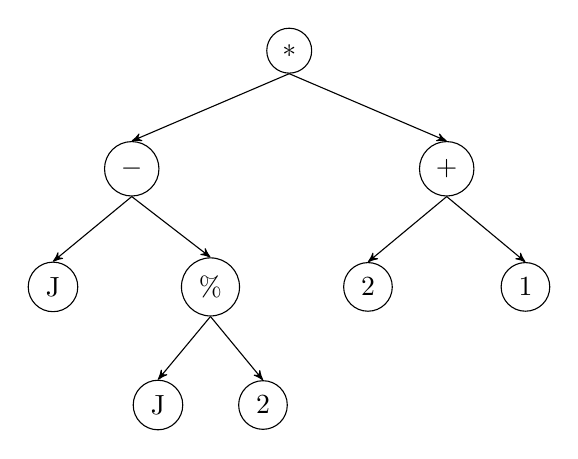
\begin{tikzpicture}[->,>=stealth',level/.style={sibling distance = 4cm/#1,
  level distance = 1.5cm}] 
\node[circle,draw](z){$*$}
 child{
    node[circle,draw]{$-$} child{node[circle,draw] {J}} child{node[circle,draw] {$\%$} child{node[circle,draw] {J}}  child{node[circle,draw] {2}}} }
  child{
    node[circle,draw]{$+$} child{node[circle,draw] {2}} child{node[circle,draw] {1}} };
\end{tikzpicture}
\end{wrapfigure}

As explained in \cite[p.19-27]{introgp} to begin designing a GP, the first step is to define the set of terminals and the set of functions, of which the program trees will be comprised of. The terminal set will be; \begin{center}$T = \{J,\ \Re\}$\end{center} $J$ as already discussed will be the value in the sequence 1 to $2^{14}$, and $\Re$ will represent a small random integer constant from the set $\{0, 1, 2, 3\}$. The set $F$ is our function or operator set; \begin{center}$F = \{+, -, *, /, \%\}$\end{center}In this set, $/$ is the protected integer quotient function and $\%$ is the protected modulus function, where both use the protected division function that returns 1 when attempting to divide by zero, and otherwise returns the normal quotient. All the terminals have an arity of 0, and all the functions have an arity of 2.

\begin{text}The next step is to define the structure of the programs. Members of the population will be represented as binary trees, in the form of prefix expressions. Take for example the expression; \end{text}
\begin{equation*}*\ -\ J\ \%\ J\ 2\ +\ 2\ 1 \end{equation*} 
This prefix expression can be represented as the binary tree in figure \ref{fig:simplebintree}. And vice versa, the prefix expression above can be generated from a pre-order traversal of the binary tree in figure \ref{fig:simplebintree}. For experimentation, the user will initially define the major parameters of the GP run. These parameters are defined in table \ref{inputparam} below;

\begin{table}[H]
\centering
\caption{Input parameters}
\label{inputparam}
\begin{tabular}{l*{6}{l}r}
Data Type             & Input description\\
\hline
Integer & Population size\\
Integer & Maximum number of generations\\
Integer & Maximum initial program depth and maximum crossover program depth\\
Double & Fitness proportionate reproduction to crossover operation balance\\
Double & Internal to external node crossover probabilities\\
Double & Target fitness value\\
\end{tabular}
\end{table}

Now we have defined the parameters, the terminals $T$, the functions $F$, and the structural representation of the programs, the next step for the GP is to use these definitions to enumerate an initial random population of programs.

Defined by the user, the GP will generate a population of the given size, where each program in the population has a maximum initial tree depth of the given size. In order to generate a wide and genetically diverse initial population, in \cite[p.11-14]{introgp} Koza suggests the even combination of both ``grow" and ``full" methods to generate program trees known as the ``ramped half and half method". This allows for a range of tree shapes and sizes all the way from a single terminal node program such as $J$, all the way up to a program which would be produced by the full function. Using this ramped half and half method, we can obtain half a population of large programs, and another half of programs with varying shapes and sizes.

Now that the GP has obtained an initial random population, it will evaluate each program and calculate it's corresponding fitness. As discussed above, the output of the RNG is a sequence of random binary digits of length $J$. To calculate the output, we must run through the sequence $J$ from $I = 1$ to $2^{14}$ substituting the occurrences of $J$ in the program with $i$. The LSB of the output given $J = i$ corresponds to the value in the binary sequence at position $i$. The GP will then calculate the binary output sequence for each RNG in the population. 

Now that the GP has evaluated every RNG, it must use a fitness function to calculate the fitness for each RNG given its respective output. In order to measure how ``random" the output is from a RNG, their are a variety of statistical and mathematical techniques at our disposal as discussed earlier. In this case, we are going to use the Shannon entropy equation from the field of Information Theory as our fitness function. The entropy of a sequence of binary digits is the equality in the occurrence of a set of binary sub-sequences of length $h$ in that sequence. The Shannon entropy calculation for all possible $2^h$ binary sub-sequences of length $h$ is;
\begin{equation*}
E_{h} = - \sum_{j} P_{(hj)}\ \log_2\ P_{(hj)}
\end{equation*}
Here $j$ ranges over all possible sub-sequences of length $h$ in the binary sequence (the RNG output in this case). In order to achieve maximum entropy for $E_h$, all probabilities for all $2^h$ binary sub sequences of length $h$ must be equal to $\frac{1}{2^h}$.

To calculate the entropy for the output of every RNG, we want to evaluate it for more than one binary sub sequence length. This is achieved by calculating the summation of the formula above for $E_h$ but over a range of lengths of $h$ from 1 to $N_{max}$; 

\begin{equation*}
E_{total} = \sum_{h = 1}^{N_{max}} \left[ - \sum_{j} P_{(hj)}\ \log_2\ P_{(hj)} \right]
\end{equation*}
The maximum possible entropy value for sub sequences from 1 to $N_{max}$ can be calculated using the following sum;
\begin{eqnarray*}
E_{max} &=& \sum_{i = 1}^{N_{max}} i
\\ &=& \frac{N_{max}(N_{max} + 1)}{2}
\\ &=& \frac{7 \cdot (7 + 1)}{2}
\\ &=& 28
\end{eqnarray*}
In this GP implementation, We shall be using sub sequences of lengths 1 to 7, so $N_{max} = 7$. This will give us the maximum entropy and therefore the maximum fitness of 28.

Now that the fitness function has been defined. The entropy for every RNG's output is calculated, for sub sequences of lengths 1 to 7.
In the C implementation, each program (RNG) will be stored in an individual struct. Each struct will contain; the RNG code/prefix expression, the program length, the output binary sequence, the scalar entropy break down for each of the sub sequence lengths of $h$ from 1 to $N_{max} = 7$ and the total fitness (the sum of these scalar entropies). So far in the design, all of these pieces of information have been defined. The population of all these structs are contained in another ``population struct" of the size defined by the user. Representing the programs and the population like this allows for easy manipulation and portability between methods in the GP.

Figure \ref{simpleflow} is a simple flow chart representation for the GP. On every round of the algorithm, data is gathered for that particular run and is saved to a text file in the format of a CSV\footnote{Where values are delimited using commas i.e. $w,\ x,\ y,\ z, ...$}(Comma Separated Values) file. Each output and it's type are defined in table \ref{outputparam} below;
\newpage
\begin{wrapfigure}[30]{h}{.4\textwidth}
\caption{GP flowchart}
\label{simpleflow}
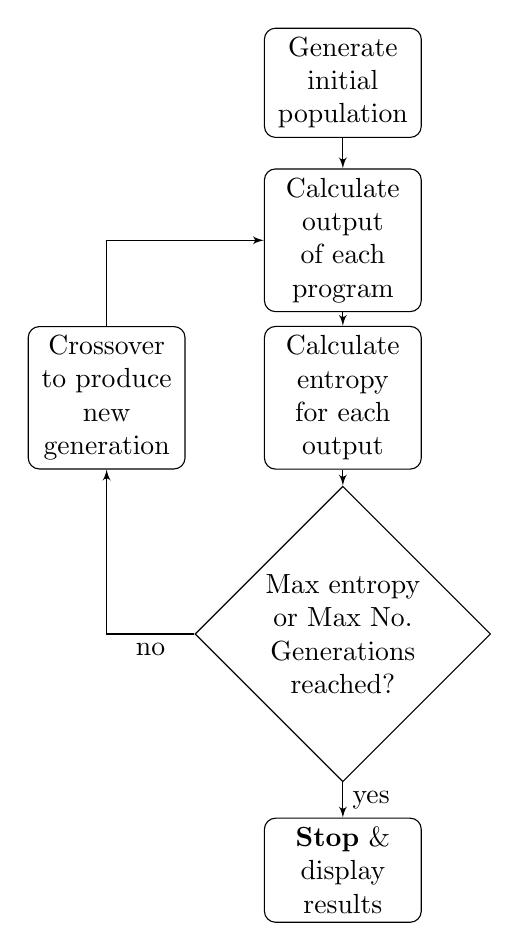
\begin{tikzpicture}[node distance = 2cm, auto]
    % Place nodes
    \node [block] (init) {Generate initial population};
    \node [block, below of=init] (identify) {Calculate output of each program};
    \node [block, below of=identify] (evaluate) {Calculate entropy for each output};
    \node [block, left of=evaluate, node distance=3cm] (update) {Crossover to produce new generation};
    \node [decision, below of=evaluate] (decide) {Max entropy or Max No. Generations reached?};
    \node [block, below of=decide, node distance=3cm] (stop) {\textbf{Stop} \& display results};
    % Draw edges
    \path [line] (init) -- (identify);
    \path [line] (identify) -- (evaluate);
    \path [line] (evaluate) -- (decide);
    \path [line] (decide) -| node [near start] {no} (update);
    \path [line] (update) |- (identify);
    \path [line] (decide) -- node {yes}(stop);
\end{tikzpicture}
\end{wrapfigure}


\begin{table}[]
\centering
\caption{Output data}
\label{outputparam}
\begin{tabular}{l*{6}{l}r}
Data Type             & Output description\\
\hline
Integer & Generation number\\
Double & Generation run time in seconds \& hundredths of a second \\
Double & Average entropy/fitness for the population\\
Double & Total entropy/fitness of fittest candidate\\
Double & Entropy for subsequence size 1 of fittest candidate\\
\ \ \ \ $\vdots$ & \ \ \ \ \ \ \ \ \ \ \ \ \ \ \ \ \ \ \ \ \ \ \ \ $\vdots$\\
Double & Entropy for subsequence size 7 of fittest candidate\\
Boolean & Entropy of fittest candidate is $\geq$ target fitness?\\
String & Prefix expression for fittest candidate\\
\end{tabular}
\end{table}


Since the design document, I have added in one extra piece of output data. This is the ``Average entropy/fitness for the population", and I included it so that during the analysis phase, I could determine how well the fitness of the population as a whole was growing and not just a single candidate. This comma separated data will be appended to the text file for each generation of the GP (each preceded with a return line character). For further information about the design of the structure of the output data, please refer to the design document in the appendix.

The final process in the GP to define is the genetic operation which shall be used. Two main genetic operators used in GP are mutation and crossover \cite[p.15-17]{introgp}. Both operate by altering program trees in different ways in order to create offspring programs. In this GP, I will be using the subtree crossover operation alone, and I will not be implementing subtree mutation in order to conserve computing time\footnote{Subtree mutation requires the generation of new subtrees which can prove to be computationally intensive, especially when mutation probability is high}.  

Subtree crossover works by taking two parent program trees and joining them to create two offspring programs. This is done by selecting a crossover point (node) in each parent tree. Both of the subtrees at the root of the crossover point are then swapped to generate the two new offspring. Crossover point selection can be at any node in the tree including leaf (in this case terminal) nodes. For this GP, one of the user inputs to the program in figure \ref{inputparam} on page \pageref{inputparam} is the probability divide of selection of internal to external nodes. In \cite[p.114]{kozagpbook}, Koza describes the benefits of using a 90\% internal (function) and 10\% external (terminal) split, saying that it ``promotes the recombining of larger structures" so that simple swapping of terminals like that of point mutation is less probable.

In table \ref{inputparam} on page \pageref{inputparam}, there is a parameter ``Fitness proportionate reproduction to crossover operation balance". This input determines the split between Fitness proportionate reproduction (FPR) and crossover.  FPR is where both parents are selected for crossover relative to their fitness. In the regular crossover selection, one of the parents is selected relative to their fitness and the other is selected with an equal probability amongst the rest of the population. The following equation calculates the selection probability for the $i^{\text{th}}$ individual in the population (used for selecting both parents in FPR and one in crossover);\\
\begin{center}
\noindent\begin{minipage}{.3\linewidth}
\begin{equation*}
p_i = \Bigg( \frac{f_i}{\sum_{x=1}^{|P|} f_x} \Bigg)
\end{equation*}
\end{minipage}%
\begin{minipage}{.2\linewidth}
where;
\end{minipage}
\begin{minipage}{.3\linewidth}
$p_i$ - selection probability of $i$\\
$f_i$ - fitness value of $i$\\
$f_x$ - fitness value of $x$\\
$|P|$  - population size
\end{minipage}
\end{center}
Now that the GP has generated a new \emph{evolved} population, it returns back to step 2 in figure \ref{simpleflow} on page \pageref{simpleflow}. This process continues until one or both of the termination criteria are met as discussed above.

Above is a literal design of the GP, covering all the major aspects of the operations. Using the definitions above, a pseudocode can be created for the key methods in figure \ref{simpleflow} on page \pageref{simpleflow} which bears a closer functional resemblance to the actual C implementation of the GP. All algorithms produced in the design process can be found in the design document. Here I only introduce the changes made and the new algorithms introduced after the design document was written. 

In algorithm \ref{fitnessfunc} we can see that a minor change has been made since the design document was written. Instead of using a brute force pattern matching algorithm, I have for the efficient finite automaton based KMP pattern matching algorithm (Named after it's designers, Knuth, Morris and Pratt). Algorithms \ref{prefixfunc} and \ref{kmpalgo} describe the two functions of this algorithm. The Compute-Prefix-Function creates a finite automaton transition function for the pattern that it is given. In essence this function calculates the earliest place in the pattern where the pattern can reoccur in itself. This way time is saved matching what has already been matched. The matching algorithm itself feeds the pattern through this automaton, keeping track of its state.

\begin{algorithm}[H]
  \caption{Compute-Prefix-Function$(j_2)$}
  \textbf{Input:} Binary pattern $j_2$.\\
  \textbf{Output:} The finite automaton mapping function $\pi$.\\
  \begin{algorithmic}[1]
	\State $m \gets $length($j_2$)
	\State $\pi[1] \gets 0$
	\State $k \gets 0$
	\For {$q \gets 2$ to $m$}
		\While {$k > 0 \land P[k + 1] \neq P[q]$}
			\State $k \gets \pi[k]$
		\EndWhile
		\If {$P[k + 1] == P[q]$}
			\State $k \gets k + 1$
		\EndIf
		\State $\pi[q] \gets k$
	\EndFor
	\State \textbf{return} $\pi$ \Comment {This algorithm returns the function $\pi$ where $\pi[q] = $max$\{k: P_k$ is a proper suffix of $P_q\}$}

  \end{algorithmic}
\label{prefixfunc}
\end{algorithm}

\begin{algorithm}[H]
  \caption{KMP-Matching$(j_2, O)$}
  \textbf{Input:} Binary pattern $j_2$ and the text (in this case binary sequence) $O$.\\
  \textbf{Output:} The number of occurrences of $j_2$ in $O$.\\
  \begin{algorithmic}[1]
  	\State $n \gets $length($O$)
	\State $m \gets $length($j_2$)
	\State $\pi \gets $Compute-Prefix-Function($j_2$)
	\State $q \gets 0$
	\State $count \gets 0$
	\For {$i \gets 1$ to $n$}
		\While {$q > 0 \land P[q + 1] \neq T[i]$}
			\State $q \gets \pi[q]$ \Comment{Using the prefix function to find the closest move backwards in the pattern we can go}
		\EndWhile
		\If {$P[q + 1] == T[i]$}
			\State $q \gets q + 1$
		\EndIf
		\If {$q == m$} \Comment {Reached the end of the pattern and therefore have a match}
			\State $count += 1$ 
			\State $q \gets \pi[q]$
		\EndIf
	\EndFor
	\State \textbf{return} $count$		 

  \end{algorithmic}
\label{kmpalgo}
\end{algorithm}

\begin{algorithm}[H]
  \caption{Fitness-Function($O$)}
  \textbf{Input:} Tree binary sequence output $O$\\
  \textbf{Output:} Fitness value $E_{total}$, and scalar entropies $E_1, E_2, ..., E_7$ corresponding to the output $O$ (which in turn corresponds to a tree/RNG)\\ 
  \begin{algorithmic}[1]
   
   \State $E_{total} \gets 0$
   \For {$h \gets 1$ to 7} \Comment{this algorithm represents $E_{total} = \sum_{h = 1}^{7} \left[ - \sum_{j} P_{(hj)}\ \log_2\ P_{(hj)} \right]$}
	\State $F \gets \emptyset$
	\State $totalOcc \gets 0$\\
	\State $j \gets 2^{h-1}$ 
	\If {$h == 1$} \Comment{we want to include 0 as a binary sequence of length 1}
		\State $j \gets 0$
	\EndIf\\
	\For {$j$ to $2^h - 1$} \Comment{this is for all numbers of binary sequence length $h$}
			\State $occurrence \gets $KMP-Matching$(j_2, O)$  \Comment Brute force algorithm replaced with KMP algorithm
		\State $F \cup \{(j_2, occurrence)\}$ 
		\State $totalOcc \gets totalOcc + occurrence$
	\EndFor
	\State $E_h \gets 0$ \Comment{calculating entropy value for subsequence size $h$}
	\For {$\forall x \in F$} 
		\State $E_h \gets E_h + \left(-1 * \left( \frac{x.occurrence}{totalOcc} \log_2 \frac{x.occurrence}{totalOcc}\right)\right) $	
	\EndFor

	\State $E_{total} \gets E_{total} + E_h$
    \EndFor
    \State \textbf{return} $E_{total}, E_1, E_2, ..., E_7$
  \end{algorithmic}
\label{fitnessfunc}
\end{algorithm}

\subsection{SNGP Approach}

The following section of this document is concerned about the design of the SNGP implementation of evolving a RNG by means of Genetic Programming. To do this, I shall be using both \cite{kozarng} by Koza and \cite{jacksonsngp2} by Jackson. This is a summary of the design, covering its most important aspects. A more elaborative description of the proposed system and examples to go along with functions can be found in the original design document in the appendix. 

Single Node Genetic Programming is similar to regular Genetic Programming in many ways, but differs in a few crucial aspects, giving rise to considerable efficiency and solution rate boosts over GP. For this reason, the design of the SNGP methodology need not be as extensive as that in section 2.1.1, but rather more to the point in terms of defining the approaches differences in comparison to GP. In \cite[p.50-51]{jacksonsngp2} Jackson describes the SNGP model in the following way;

A population is a set $M$ of $N$ members where;
\begin{center}
$M = \{m_0,\ m_1,\ ...,\ m_{N-1}\}$
\end{center}
Each member $m_i$ is a tuple;

\begin{center}
\noindent\begin{minipage}{.5\linewidth}
\begin{equation*}
m_i = \ <u_i,\ r_i,\ S_i,\ P_i,\ O_i>
\end{equation*}
\end{minipage}%
\begin{minipage}{.4\linewidth}
$u_i \in \{T \cup F\}$ - node in the terminal or function set\\
$r_i$ - fitness of the node\\
$S_i$ - set of successors of the node\\
$P_i$ - set of predecessors of the node\\
$O_i$ - output vector for this node\\
\end{minipage}
\end{center}

This tuple will be adapted into a $struct$ in C like the GP program described above.

For this implementation, I will be adapting the fitness value $r_i$ into a vector $R_i$ \footnote{So that the output of the SNGP will be the same as the GP, giving me the option to compare approaches on scalar entropies}. The first element in the vector will be the total fitness $E_{total}$ and the rest of the elements will be the scalar entropy values from $E_1$ to $E_7$.

SNGP is node focused, this means that members of the population are not trees, but are single nodes which together create a larger graph structure.

\begin{wrapfigure}[44]{h}{.4\textwidth}

\caption{SNGP flowchart}
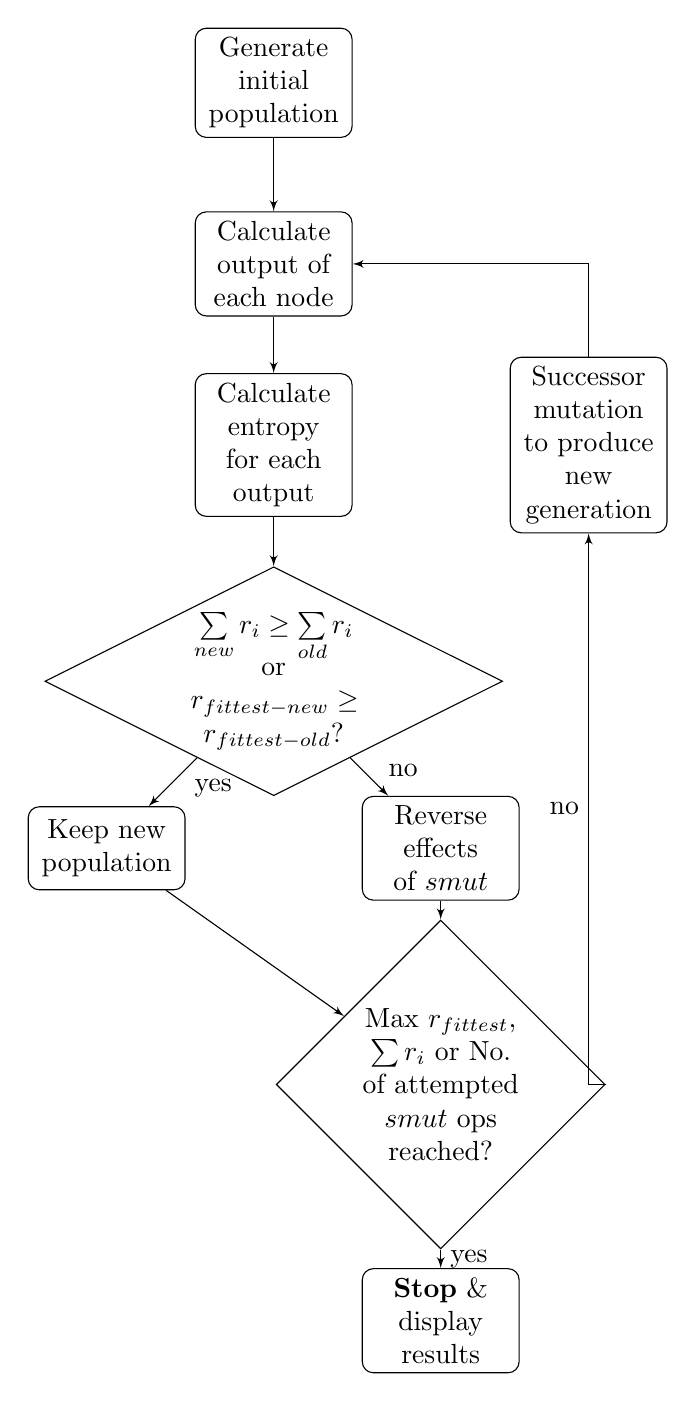
\begin{tikzpicture}[node distance = 2.3cm, auto]
    % Place nodes
    \node [block] (init) {Generate initial population};
    \node [block, below of=init] (identify) {Calculate output of each node};
    \node [block, below of=identify] (evaluate) {Calculate entropy for each output};
    \node [block, right of=evaluate, node distance=4cm] (update) {Successor mutation to produce new generation};
   
 \node [draw, decision, aspect=2,  below of=evaluate] (decide1) {$\sum\limits_{new} r_i \geq \sum\limits_{old} r_i$ or ${r}_{fittest-new} \geq {r}_{fittest-old}$?};
    \node [block, below left of=decide1, node distance=3cm] (greater) {Keep new population};
   \node [block, below right of=decide1, node distance=3cm] (less) {Reverse effects of $smut$};
    \node [decision, below of=less] (decide2) {Max $r_{fittest}$, $\sum r_i$ or No. of attempted $smut$ ops reached?};
    
\node [block, below of=decide2, node distance=3cm] (stop) {\textbf{Stop} \& display results};
    % Draw edges
    \path [line] (init) -- (identify);
    \path [line] (identify) -- (evaluate);
    \path [line] (evaluate) -- (decide1);
    \path [line] (decide1) -- node  [near start]{yes} (greater);
    \path [line] (decide1) -- node [near end] {no} (less);
    \path [line] (less) -- (decide2);
    \path [line] (greater) -- (decide2);
    \path [line] (decide2) -| node [near end] {no} (update);
    \path [line] (update) |- (identify);
    \path [line] (decide2) -- node {yes}(stop);
\end{tikzpicture}
\label{simpleflowsngp1}
\end{wrapfigure}



Figure \ref{simpleflowsngp1} shows a flowchart for the anticipated SNGP implementation. Here we can see that the main functions are similar to those of GP.
In SNGP, the initial population is also randomly generated but instead, members of the population are chosen as individual nodes.

The Inputs to the SNGP implementation are shown in table \ref{inputparamsngp} on page \pageref{inputparamsngp}. There are less inputs for the SNGP implementation compared to the conventional GP implementation. The length of a run is the equivalent to the maximum number of generations for GP, where instead the program terminates after a certain number of attempted successor mutation operations. This has been changed since the original design document. Initially termination was designed to end on the number of successful $smut$ operations. It has since been changed to the number of attempted operations in order to bring fairness between GP and SNGP implementations. The terminating fitness value is taken from the sum of all fitness values in all the nodes of the population, or upon finding a solution (a root node representing a tree with an entropy greater than 27.990 bits). This has also been changed since the original design document, upon realisation that a single solution is desired. The population size is the number of nodes in the SNGP graph population. This size remains constant from initial generation throughout the rest of the run.

The SNGP population differs from the tree structure of a single member in the GP population. While the arity of functions and terminals remain the same as of that in the GP implementation, each function and terminal may have more than one predecessor. Therefore every node in the population can act as a root node for a RNG, and a population therefore contains as many RNGs as there are nodes. The reason for this coming about is due to the way that the population is initialised and evolved.

To begin with, all of the terminals in $T$ are added to the population exactly once. From here on in over all the generations, these terminals remain the same. What changes are their predecessors. Once the terminals are added, the functions are now selected randomly and are added to the population where their operands are existing members of the population. During initialisation of the population, the output and the fitness of each individual is also assessed. As Jackson describes in \cite[p.52]{jacksonsngp2}, this is what gives rise to SNGPs efficiency.

As the first terminals are added, they are evaluated for their outputs and their fitness is subsequently calculated. In this implementation of SNGP, this process is almost identical to that of the GP implementation described above. The terminal is evaluated for all values of $J$ from $i = 1$ to $2^{14}$, and each output is stored in the vector $O_i$ for that node. From this output vector a binary sequence of length $J$ is generated from the LSB of each element in $O_i$. The fitness of that node is the total entropy for subsequence's of length 1 to 7 in the binary sequence, using the same equation as in the GP approach;
\begin{center}
 $E_{total} = \sum_{h = 1}^{7} \left[ - \sum_{j} P_{(hj)}\ \log_2\ P_{(hj)} \right]$
\end{center} 

This fitness/entropy value is stored in $r_i$ for that node. The efficiency of SNGP arises from using the following form of dynamic programming; when functions are now added to the population and their successors are assigned, the output and fitness for these nodes are calculated from the output vectors of their successors in the set $S_i$, as opposed to calculating them from scratch.

In SNGP, evolution is driven by hill-climbing. This is that the fitness is taken as the sum across the whole population; $\sum r_i$. After evolution this sum is calculated again, and if it is greater (higher entropy) than the last, then this evolved population replaces the previous population, otherwise the old population is kept and the process is repeated. I have changed the original design so that it is also driven on an increasing fittest member of the population. This way, it is easier to focus the evolution on trying to produce a solution as well as an entire graph with a high fitness. 

\begin{table}[H]
\centering
\caption{Input parameters}
\label{inputparamsngp}
\begin{tabular}{l*{6}{l}r}
Data Type             & Input description\\
\hline
Integer & Length of a run (number of attempted $smut$ operations)\\
Integer & Population size (number of nodes)\\
Double & Total (i.e. sum of) target fitness value\\
\end{tabular}
\end{table}

Evolution of a SNGP is not done by using the crossover operation like in the GP above, but instead uses the $smut$ or successor mutation operation. A member of the population (a node) is randomly selected, and one of the members in it's successor set is changed to another member of the population (still at a greater depth in the tree). 

During $smut$, not all of the program nodes are effected, and therefore not all of them need to be re-evaluated for their outputs and fitnesses. As Jackson describes in \cite[p.53]{jacksonsngp} SNGP that retains it's efficient nature by creating an update list, where only nodes effected by smut are added. Nodes in the list are re-evaluated starting at the lowest node in the list working up to the highest node so that no node is revisited.

The outputs for the SNGP implementation are almost identical to those of the GP. Instead of Generation Number, the output here will be the $smut$ operation count. Like the GP implementation I have also added the average fitness of the members of the population as an output. Please see the design document in the appendix for further detail on output data for the SNGP implementation.

Since the design document was produced, no changes have been made to the algorithms for the SNGP apart from the fitness function using the KMP matching algorithm, which is shown in algorithms \ref{fitnessfunc}, \ref{prefixfunc} and \ref{kmpalgo} in the design documents on pages \pageref{kmpalgo} and \pageref{fitnessfunc}. Please see the design document in the appendix for the algorithms specific to the SNGP implementation.

\newpage
\section{Implementation}
In this section I shall cover the transition I made from design into executable code. I shall cover the GP and SNGP implementations, as well as the program I produced in order to assess the C RNG and the TRNG at random.org. As I created all of the main methods / algorithms in the design stage, the main body of implementation was to take the pseudo code and change it into C syntax. Code listings can be found in the appendix of this report, but the important functions of all approaches (algorithms in the design document implemented into code) will be described in code in this section.

\subsection{GP Implementation}

\subsubsection{Main Data Structures}
The first thing that I did when I started the implementation stage was to define the primitive objects to be used and manipulated by the algorithms described in the design section. Specifically these were the set of functions and terminals that make up the tree structure, and also the structure which holds all the information about each member of the population.

I combined the set $T = \{J,\ \Re\}$ of terminals and the set $F = \{+, -, *, /, \%\}$ of functions into a struct of tokens, each token was also a struct containing two bits of information;

\begin{lstlisting}[language=C]
struct token_entry {
   char *name;
   int arity;
};
\end{lstlisting}

The name denotes the character representation of the node, and the arity represents the number of children nodes or operands that each node has. If the node is a terminal then it will have an arity of -1, if it is a function it will have two children and therefore an arity of 1 (including 0 in the arity).

All the tokens needed to represent the RNG trees as prefix expressions are then encapsulated into an array of tokens;
\begin{lstlisting}[language=C]
struct token_entry token_table [] = {{"#", -1}, {"J", -1}, {"R", -1}, {"+", 1}, {"-", 1}, {"*", 1}, {"%", 1}, {"/", 1}, {"0", -1}, {"1", -1}, {"2", -1}, {"3", -1} };
\end{lstlisting}

The next step was to describe each member in the population as some data structure. Every member has it's own specific information. As discussed in the design section (and more extensively in the design document in the appendix).

\begin{lstlisting}[language=C]
struct population_member {
   char code[MAX_PROG_SIZE + 1];
   char output[J + 1];
   int proglen;
   double scalar_entropy[H_MAX];
   double total_fitness;
};
\end{lstlisting}

Every member in the population has it's own code (RNG tree represented as a prefix expression), binary output, length of the code, scalar entropy of the output and total fitness. These are all therefore encapsulated in the struct as seen above. A population of these structs is then formed by creating a struct of a defined population size which embodies them all;

\begin{lstlisting}[language=C]
struct population_member population[POP_SIZE];
\end{lstlisting}

\subsubsection{Generating Initial Population}
In order to obtain a full population that can be tested and evolved we must randomly generate an initial population of RNG trees. These trees as discussed are to be represented in a prefix expression so that they can be easily stored in a character array but interpreted and manipulated as trees. The following generate\_initial\_pop method is called at the beginning of the programs execution. As discussed earlier and in \cite[p.11-14]{introgp}, Koza suggests the use of the ``\emph{ramped half and half}" method. This meaning that half of the trees are created as full trees (right up to the depth limit) and the other half with as grow trees (terminals are added in randomly and not just at the depth limit). I implemented my initial population function in the same way and also with an increasing depth limit from a depth of 2 up to the user defined maximum initial depth. This gives us a diverse initial population of trees of varying shapes and sizes.

The following generate\_initial\_pop method controls the parameters for the tree types. The full integer is equal to the population member number modulus 2. This means that it alternates between 0 and 1, and therefore indicating whether the tree should be made using the grow or full method to the create\_tree function. The depth integer controls the depth limit of the trees created. This process is partitioned into groups of different tree depths;
\begin{lstlisting}[language=C]
void generate_initial_pop() { 
  struct population_member *progp = population;
  int i, j, depth, full;
  char *end_tree;

  char* text = "Generating init pop: ";

  for (i = 2; i <= MAX_INIT_DEPTH; i++) {
     for (j = 0; j < PARTITION_SIZE; j++)  {  
        full = j%2; //Half full and half grow
        depth = i;
        end_tree = create_tree(progp->code, depth, full);
        //Create tree up to ``depth" with alternating full and grow.
        end_tree = '\0';
        progp->proglen = strlen(progp->code);
        if (depth < MAX_INIT_DEPTH) 
            depth++;
        progp++;
     }
   print_progress(text, i, 50, MAX_INIT_DEPTH);
  }
}
\end{lstlisting}

In this method, the population is enumerated with trees by calling the create\_tree method. The type and depth of the trees are controlled in this method, but the tree/RNG code is created in the create\_tree method. The implementation of this method can be seen below. If the depth is 1 then then a terminal must be added, and if the value is R then this is replaced with a random integer constant from the set \{0, 1, 2, 3\} and is then added to the tree code. Otherwise, as discussed above, depending on the value of the full integer the token is chosen from the set of functions (if it is full) or from the set of both functions and terminals. Branches are then recursively created depending on the arity of the chosen node value. This is done with decreasing depth, as to eventually reach the depth of 1 where terminals are added instead of functions.

\begin{lstlisting}[language=C]
char *create_tree(char *tree, int depth, int full) { 
   char token; int arity_m1, i;
   if (depth == 1) {
      token = random_terminal();
	  if (strcmp(token_table[token].name, "R") == 0) {
		  token = random_r(); //If the token is R then assign a random variable, either 0, 1, 2 or 3
	  }
	  *tree++ = token; //Add the token to the code
   }
   else { 
	  token = (full ? random_function() : random_token()); 
	  //If full is equal to 0 then function is chosen, otherwise any token from F and T can be chosen
	  if (strcmp(token_table[token].name, "R") == 0) {
		  token = random_r(); 
 		  //If the token is R then assign a random variable, either 0, 1, 2 or 3
	  }
	  *tree++ = token;
      arity_m1 = token_table[token].arity;
      for (i=0; i <= arity_m1; i++) //If token is a function then extra branches are created
         tree = create_tree(tree, depth-1, full);
   }
   return(tree);
}
\end{lstlisting}

From these functions, I was able to obtain an inital population. I used print statements during development of these functions in order to see that the trees being created were in fact correct and diverse.
\subsubsection{Evaluating Trees}
After implementing the functions that generate a random initial population, the next phase (referring to the flow chart in figure \ref{simpleflow} on page \pageref{simpleflow}) was to write a method to evaluate / calculate the output of these tree's. Taking the algorithm from the design section I was able to implement the following method for recursively conducting a pre-order traversal of the RNG expressions, applying the operations at the functions in the branches to the terminals that are returned at the leaf nodes of the tree;

\begin{lstlisting}[language=C]
long calculate_tree_output() {
	char code_token = *prog_code++;
	char token = *token_table[code_token].name; 
	switch(token) {
		case '+': return(calculate_tree_output() + calculate_tree_output());
		case '-': return(calculate_tree_output() - calculate_tree_output());
		case '*': return(calculate_tree_output() * calculate_tree_output());
		case '%': return(protected_mod(calculate_tree_output(), calculate_tree_output()));
		case '/': return(protected_div(calculate_tree_output(), calculate_tree_output()));
		case 'J': return(current_j);
		default: return(token-'0'); //Must be R = {0, 1, 2, 3} 
	}
}
\end{lstlisting}

During implementation, for my protected mod (and division) functions I was returning the following statement (if $dom$ is not equal to 0); 

\begin{lstlisting}[language=C]
return (num%dom);
\end{lstlisting}

On some runs I was getting an Integer overflow error. At the time I was using integers. I changed them to the long data type, and noticed I was still getting the same error on occasion but still for Integers. Upon some research I found that if both values (despite being longs) are not casted as them, then C will conduct Integer arithmetic operations on them regardless. I then changed the return statements to;

\begin{lstlisting}[language=C]
return ((long)num%(long)dom);
\end{lstlisting}
\noindent and haven't since had the error message.

The method which calls this method does so by cycling through the sequence J from 1 to 16834. The current\_j variable above is a global integer variable which is set by this higher up method. The output from the calculate\_tree\_output method populates that individuals binary output array by using the modulus function seen below;

\begin{lstlisting}[language=C]
long output_for_j = calculate_tree_output();
int lsb = output_for_j % 2;
if (lsb == 0) 
   progp->output[x] = '0';
else
   progp->output[x] = '1';
\end{lstlisting}

This process is repeated for every integer in the sequence of 1 to 16834 and for every member of the population. After this has been done, every member of the population will have it's own corresponding output sequence, ready for it's entropy / fitness to be calculated. 
\subsubsection{Fitness Function}
In this section I show the transition I made from the pseudo code definition of the fitness function in the design section into a method that is used to assess the entropy and therefore fitness of each member of the population. To recap, the equation below is used in order to calculate the entropy of a binary sequence for subsequences of length 1 to $N_{max}$;

\begin{equation*}
E_{total} = \sum_{h = 1}^{N_{max}} \left[ - \sum_{j} P_{(hj)}\ \log_2\ P_{(hj)} \right]
\end{equation*}

Therefore to implement this in code the method should first cycle through all subsequences of length 1 to $N_{max}$ and count their occurrences in the binary sequence. This is done using the KMP\footnote{Knuth Morris Pratt - finite automaton based pattern matching} pattern matching algorithm. As discussed in the revised design, I replaced the initial brute force pattern matching algorithm in order to make the fitness function more efficient. The algorithm is called like so, where j2 is the padded\footnote{Including preceding zeros} binary subsequence to be searched for (i.e. the pattern), and bit\_seq is the binary output of the current program;
\begin{lstlisting}[language=C]
occurrence = KMP_matching(j2, bit_seq);
\end{lstlisting}

The occurrences are then entered into an array for that specific sequence, and the total occurrence is incremented by the same amount;
\begin{lstlisting}[language=C]
occurrence_array[array_count] = occurrence;
array_count++;
total_occ += occurrence;
\end{lstlisting}

Once this has been done for every binary subsequence of lengths 1 to H\_MAX (In our case defined as 7), then we can calculate the scalar entropy for each specific subsequence length. In the part of the fitness function below, the probabilities of occurrence of each subsequence are calculated by dividing the occurrence of that subsequence by the total occurrence for that length. The inner section of the equation above is then calculated and the scalar entropy for that length is then incremented by the entropy for that specific binary subsequence. This process is repeated for every element of ocurrence\_array (i.e. every subsequence of that length) and then this is repeated for every length to obtain all the scalar entropies;

\begin{lstlisting}[language=C]
for (int z = 0; z < array_count; z++) {
   int occ = occurrence_array[z];
   double prob = 0;

   if (total_occ != 0) 
      prob = occ / (double)total_occ;

   double e_h_increment;
   //Avoid log(0) and negative zero
   if (prob == 0 || prob == 1) 
      e_h_increment = 0;
   else
      e_h_increment = (-1*((prob*log10(prob))/log10(2.0)));
   e_scalar[h - 1] = e_scalar[h - 1] + e_h_increment;
}
\end{lstlisting}

The scalar entropies are then copied over to the scalar array of that program and then summed to obtain the full entropy/fitness value. This process of assessing the fitness is repeated for every program in the population.

When I first implemented the fitness function, I noticed I was not achieving the desired fitness levels. I initially thought that it was down to a bad population. I then used the prefix expression that Koza provides as his fittest solution in \cite{kozarng} as a test case, with a known fitness of 27.996 bits. I noticed that was only achieving around 15 bits of entropy. From this I knew that it was down to either the evaluation method or some component of the fitness function. I then realised that I was overlooking binary subsequence patterns with preceding zeros, (i.e. For length 2 for example I was checking the occurrences of 0, 1, 10, and 11 when in fact I should have been checking the occurrences of 00, 01, 10 and 11). Once I noticed this, I implemented a method that added the correct number of preceding zeros to each sequence. I then tested Koza's solution again and got exactly the same entropy as he did. I knew then that my fitness function was correct.

\subsubsection{Evolution}
For the GP implementation the only evolutionary operator I used is genetic crossover. As I Koza discussed in \cite{kozarng} and I described in the design section, for selection, we use FPR (Fitness Proportionate Reproduction) and then the rest uses equal selection with one parent selected based on their fitness. The balance between the two is defined by the user (as a definition in the code).

For FPR, the fitnesses of the population are summed and then a random number is chosen in the sums range;
\begin{lstlisting}[language=C]
//Adding POP_SIZE so that programs with 0 entropy still have chance
double total_select = fitness_sum + POP_SIZE; 
double selection = ( (double)rand() * total_select ) / (double)RAND_MAX;
\end{lstlisting}

The population fitnesses are then summed until the random number falls in between the current nodes fitness. Thus giving fitter members a greater chance of being selected. Below, the ineteger s is the index in the population array of the member chosen.

\begin{lstlisting}[language=C]
int fpr_selection() {
  double total_select = fitness_sum; //Adding POP_SIZE so that programs with 0 entropy still have chance
  double selection = ( (double)rand() * total_select ) / (double)RAND_MAX;
  for (s = 0; s < POP_SIZE; s++) {
     struct population_member *progp = &population[s];
     acc_fitness = acc_fitness + 1 + progp->total_fitness;
     if (acc_fitness >= selection && selection >= old_acc_fitness) {
        break;
    }
}
\end{lstlisting}

When calling this method, for the split of our FPR seclection is conducted like so;

\begin{lstlisting}[language=C]
do{
   parent_a = fpr_selection();
   parent_b = fpr_selection();
} while(parent_a == parent_b);
\end{lstlisting}

The rest of the selection is then done, as mentioned above, with one parent selected based on their fitness and the other with equal probability across the population;

\begin{lstlisting}[language=C]
do {
   parent_a = fpr_selection();
   parent_b = rand()%POP_SIZE;
} while(parent_a == parent_b);
\end{lstlisting}

The crossover points in both parents are then selected. To begin with, the variable node\_type, a random rational natural number greater than 0 and less than 1 is created. If it is less than the user defined INTERNAL\_NODE\_PROB (which is also a rational natural number greater than 0 and less than 1) then an internal node is selected from that parent, otherwise a terminal / leaf node is selected;

\begin{lstlisting}[language=C]
if (node_type <= INTERN_NODE_PROB && progp->proglen != 1) {
   char token;
   do{
      crossover_point = rand()%progp->proglen;
      token = progp->code[crossover_point];
   } while(token_table[token].arity != 1);
}
else {
   char token;
   do{
      crossover_point = rand()%progp->proglen;
      token = progp->code[crossover_point];
   } while(token_table[token].arity != -1);
}
\end{lstlisting}
This method is then called for both parents in order to select crossover points. 

Now that I have implemented the selection of the parents and the nodes within each of those parents, the next step is to create two child programs from them.
The code for creating the two children from the parents can be found in the appendix. It is a simple case of copying over the code from the two selected points into two new char arrays, but is long winded. This process is then repeated for a total of half the size of the population (each reproduction produces two child programs).

The main method of the program controls the calling and amalgamation of all the methods mentioned above. The main method repeats the process of evolving the population until the terminating criteria is met (entropy threshold reached or max number of generations reached). This is then repeated some number of times defined by the user, for conducting more runs and gathering larger amounts of data for testing purposes. The main method also implements a clock function which records the amount of time each run and generation takes. All of the information is written to multiple and individual run log files. Other (non major) methods and the rest of the code can be found in the appendix at the end of this document. 



\subsubsection{Conclusion}
At the end of the GP implementation I had obtained a working command line based Genetic Program which evolves RNGs. It is adaptive to experimentation as all parameters of the run can be altered in the code and data from each run describing each generation is written to log files on the hard drive. Having completed this, I now had a strong basis for beginning the SNGP implementation and for collecting data about the GP performance for later evaluation. Figure \ref{gpss} shows a screen shot of the GP running in the command line;

\begin{figure}[H]
\centering
\caption{GP Screen Shot}
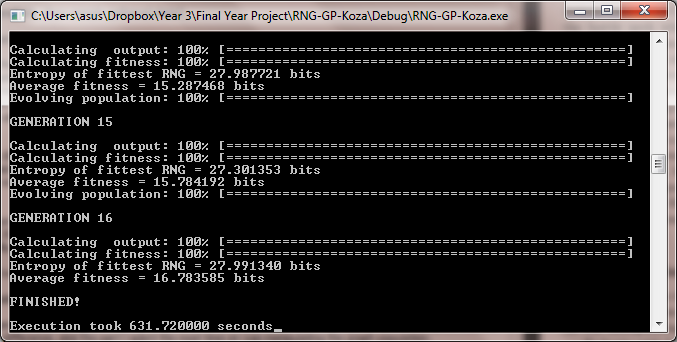
\includegraphics[scale = 0.75]{gp-ss.png}
\label{gpss}
\end{figure}


\subsection{SNGP Implementation}
In this section I shall cover the process of implementing the SNGP paradigm of genetically breeding a RNG. As the aim of the completed program is to search for optimal RNGs in the same way as the GP implementation, a lot of the methods are the same including the fitness function. What differs between the two implementations is that SNGP handles a graph population instead of separated trees, and evolves and evaluates them using dynamic programming.

\subsubsection{Main Data Structures}
 In the design section and in \cite[p.50-51]{jacksonsngp2} Jackson describes the SNGP model in the following way;

A population is a set $M$ of $N$ members where;
\begin{center}
$M = \{m_0,\ m_1,\ ...,\ m_{N-1}\}$
\end{center}
Each member $m_i$ is a tuple;

\begin{equation*}
m_i = \ <u_i,\ r_i,\ S_i,\ P_i,\ O_i>
\end{equation*}

I implemented these tuples as structs in C. Here we can see how each node is described as a struct in C for the SNGP implementation.

\begin{lstlisting}[language=C]
struct population_member {
   char node_value;
   int depth;
   long dec_output[J];
   char bin_output[J + 1];
   int pred[POP_SIZE]; //1 if node index is predecessor
   int suc_1; //Array index of left successor
   int suc_2; //Array index of right successor 
   double scalar_entropy[H_MAX];
   double total_fitness;
};
\end{lstlisting}

As each of these structs represents a node in a graph population, information on the nodes position is needed. Therefore I added some extra data from the GP struct. The depth of the node is important for evolution purposes, as to ensure that nodes cannot mutate to other nodes higher up or equal to the depth they are at (this could cause a cycle in the graph leading to infinite trees being created). Each node can have any number (up to POP\_SIZE - 1) of predecessors, therefore the pred integer array stores the index of these predecessors. This is later used for creating update lists after evolution. Each function has two successors, the index of which are stored as integers in the struct. The decimal output vector is also needed in order to conduct dynamic calculations during evaluation.

A graph of these struct descriptions of the nodes is formed by creating a larger struct to embody them all;

\begin{lstlisting}[language=C]
struct population_member graph[POP_SIZE];
\end{lstlisting}

\subsubsection{Generating Initial Population \& Evaluation}
The next stage was to write a method to populate this graph struct, called at the beginning of the programs execution. Every terminal node is added to the graph first. Terminals have no successors, and their outputs are calculated as they are added to the graph. For the J terminal, the output is 1 to 16834. For all the other terminals (i.e. $\Re = \{0, 1, 2, 3\}$) their output is an array of the terminal values (so for 0 it is an array of 16834 0's). Functions are now added to the graph, selecting successors at random. The outputs for the function nodes are also calculated as they are added to the graph, taking the outputs of the left and right hand sucessors output array at every index (through the sequence) and applying the function to these two values.


For terminals, in the code we add their values to their output array;
\begin{lstlisting}[language=C]
current_j = x + 1;
if (*token_table[curr_node->node_value].name == 'J') {
	output_for_j = current_j;
}
else if (*token_table[curr_node->node_value].name == '0') {
	output_for_j = 0;
}
else {
	output_for_j = *token_table[curr_node->node_value].name - '0'; 
}
curr_node->dec_output[x] = output_for_j;
\end{lstlisting}

This is done for every $current\_j = 1 \to 16834$. The binary array is then populated by taking the LSB of this output.

For functions, the output is calculated by taking the left and right hand nodes output and applying the operation to them;

\begin{lstlisting}[language=C]
struct population_member *node_left = &graph[curr_node->suc_1];
struct population_member *node_right = &graph[curr_node->suc_2];
\end{lstlisting}

The following code is the case statement for the multiplication function. The other case statements are similar in structure but they apply their corresponding operation to the two decimal values;

\begin{lstlisting}[language=C]
case '*': 
   for (int i = 0; i < J; i++) {
       curr_node->dec_output[i] = node_left->dec_output[i] * node_right->dec_output[i];
       if ((curr_node->dec_output[i] % 2) == 0) 
         curr_node->bin_output[i] = '0';
       else
         curr_node->bin_output[i] = '1';        
   }
   break;
\end{lstlisting}

This process is repeated for any new node added to the graph population during it's initialisation. However, as we will see below, in later generations when the graph is updated after a mutation, not every node needs to be updated.

\subsubsection{Successor Mutation /  Evolution}
The only evolutionary operator I used in the SNGP implementation (and described by Jackson on \cite{jacksonsngp}) is successor mutation or $smut$. A node is chosen at random (minus the terminals), and one of it's successors is mutated to some other node in the graph (still at a lower depth). The implementation of this function was relatively simple as it purely relies on random selection and updating of the nodes involved.;


\begin{lstlisting}[language=C]
int mut = (rand() % (POP_SIZE - NUM_TERMINALS)) + NUM_TERMINALS; //Randomly pick node in graph (excluding terminals)
int suc = rand() % 2; //Left or right hand successor

...

do {
   mut_to = rand() % mut;
   mut_to_node = &graph[mut_to];
} while (mut_to == current_suc_1 && mut_to_node->depth >= mut_node->depth);

mut_node->suc_1 = mut_to;
mut_to_node->pred[mut] = 1;
\end{lstlisting}

The nodes depth is then updated by taking the successor with the greatest depth and adding 1;

\begin{lstlisting}[language=C]
if (left->depth >= right->depth)
		mut_node->depth = left->depth + 1;
	else
		mut_node->depth = right->depth + 1;
\end{lstlisting}

The tricky part was to create an update list. After the successor mutation operation, the only nodes that need to be updated are the ones which are it's predecessors and the predecessors. Therefore I needed to create a recursive algorithm that backtracked through the graph in order to create an update list.

First I wrote the following method to initialise the update list;


\begin{lstlisting}[language=C]
void init_update_list() {
	for (int x = 0; x < POP_SIZE; x++) {
		update_list[x] = -1;
	}
}
\end{lstlisting}

Then I created the following method to create the update list. Given the index of the node which has been updated, the method is then called recursively on the parent nodes.
\begin{lstlisting}[language=C]
void create_update_list(int update_node) {
	//Only need to update the predecessors of the 
	struct population_member *curr_update = &graph[update_node];

	for (int i = 0; i < POP_SIZE; i++) {
		if (curr_update->pred[i] == 1) {
			if (update_list[i] != 1) { //Adding to list (only counting repeated nodes once)
				update_list[i] = 1;
				update_size++;
			}
			create_update_list(i); //Recursively calling on predecessors
		}
	}
}
\end{lstlisting}

After implementing this I had complete code for running one generation. The rate at which the SNGP implementation evolved was alarming at first having been used to the slower GP. I was able to build around these methods in the main method in order to create runs.
\subsubsection{Other Methods and Conclusion}
During implementation I experimented with various combinations of driving factors. In SNGP the most effective climbing approach I found was to drive on either the increase of the total population fitness or on the fittest members fitness increase;
\begin{lstlisting}[language=C]
if (best_fitness_old >= best_fitness && total_pop_fitness_old >= total_pop_fitness)
{
 //Then throw away new graph population after mutation
}
\end{lstlisting}

I then implemented the termination criteria using simple variables and conditional statements. Since the design document and during implementation I changed the termination criteria with regards to mutations from the number of actual mutations to the number of attempted mutations. As Jackson describes in \cite{jacksonsngp} this gives a fairer comparison against the number of individuals processed in the GP implementation.

After this, I was then able to start conducting runs and writing test data. The code for writing data is simple and can be found in the appendix along with the rest of the code for the SNGP implementation. It simply writes the run data to a text file in the format mentioned in the design document in the appendix. The files produced are named according to the time at which the run was started.

Having completed these tasks, I had a fully operating SNGP solution ready for testing and evaluation. At this point I was confident about the work I had done, and also about the outcome of the evaluation of SNGP vs GP due to the runs that I had already collected through testing both implementations. Figure \ref{sngpss} below is a screen shot from an example run of the SNGP paradigm.

\begin{figure}[H]
\centering
\caption{SNGP Screen Shot}
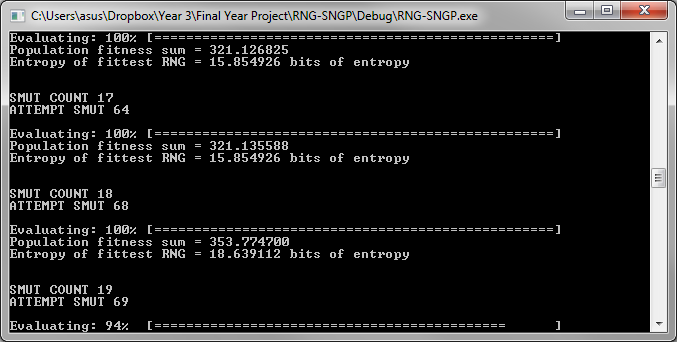
\includegraphics[scale = 0.75]{sngp-ss.png}
\label{sngpss}
\end{figure}

\subsection{C $rand()$ and TRNG Test Program Implementation}
Having implemented both the GP and SNGP paradigms ready for being run and to have data collected, the next and final implementation stage was to write a piece of software in C that would test both the C RNG and the TRNG in the same way that the RNG trees are tested in GP and SNGP.

I set out knowing that the fitness function from the GP and SNGP implementations would need to be used identically. Therefore all I needed to do for both the C $rand()$ function and the TRNG at random.org was to collect their binary outputs and populate an array of length 16834. This array can then be tested in the same way in order to produce a fair test.
\subsubsection{C $rand()$}
I began by implementing some user definitions. When the program is executed, the user is prompted to decide which method should be assessed. If `c' is pressed then the user is again prompted for the number of runs they would like to conduct. This was implemented using simple $getch()$ and $scanf()$ method calls (i.e. get char). Once I had this working, the following method is called;

\begin{lstlisting}[language=C]
void get_c_rand_seq() {
   for (int i = 0; i < J; i++) {
    int bit = rand()%2;
    if (bit == 0)
      bit_seq[i] = '0';
   else 
      bit_seq[i] = '1';
   }
}
\end{lstlisting}

Here I took the remainder of dividing the output of the C $rand()$ function by 2 (mod function, so output is 0 or 1), and populated the bit\_seq character array.

This bit sequence is then assessed using the Shannon entropy equation (from the fitness function) and the program outputs the average (from the user defined number of runs) entropy value and percentage on screen, out of 28 bits (or the max entropy for the defined H\_MAX). The run information, consisting of the run number and scalar entropy breakdowns, are then saved into a log file on the hard disk so that it can be used for evaluation purposes.

A screen shot of the C $rand()$ implementation can be seen below;

\begin{figure}[H]
\centering
\caption{C $rand()$ Screen Shot}
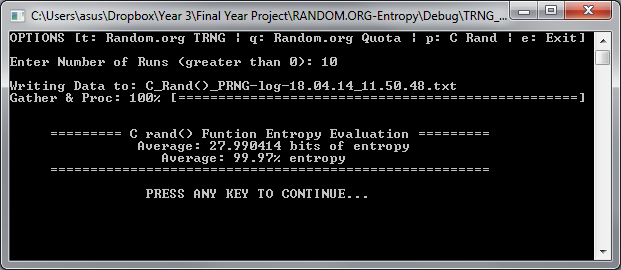
\includegraphics[scale = 0.75]{c-ss.png}
\label{sngpss}
\end{figure}


\subsubsection{Random.org TRNG}
The other option when the user is prompted is to test the TRNG at Random.org. The same Shannon entropy equation (i.e. fitness function) is used to keep the evaluation of the methods fair. 

In order to retrieve a random bit sequence from the random.org servers I had to call the following HTTP request and save the file to disk (deleting the old one from the cache so that we don't get the same sequence twice).

\begin{lstlisting}[language=C]
void download_bits() {
	HRESULT hr;
	LPCTSTR Url = _T("http://www.random.org/cgi-bin/randbyte?nbytes=2048&format=b.txt"), File = _T("RandomBits.txt");
	DeleteUrlCacheEntry(Url);
	hr = URLDownloadToFile (0, Url, File, 0, 0);
}
\end{lstlisting}

In the HTTP request the nbytes varaible is the number of bytes I want to download. As the binary array is 16384 bits long, I want 16384/8 = 2048 bytes. I also want the it to be in bit form (i.e. base 2) and I want it to be text file, hence the format parameter `b' and the final .txt extension are added to the request. 

Once the file has been downloaded, the binary data is be read into a char array and then the entropy of the sequence is calculated. The code for reading in from the RandomBits.txt file ca be seen below. 

\begin{lstlisting}[language=C]
for (position; position < J; position++) {
			c = getc(file);

			while (c != '1' && c != '0')
				c = getc(file);
			bit_seq[position] = c;

		}
		//printf("POSITION: %d\n", position);
		bit_seq[J] = '\0';
\end{lstlisting}

Originally I was reading in all of the sequence except for spaces and `\textbackslash n' characters. I then noticed that there were other hidden characters I was not compensating for including return line statements (i.e. `\textbackslash r'). I changed the code so that any character that is not a 1 or a 0 is skipped. As a result I began achieving slightly higher (and correct) entropy values.

Like the C implementation this process is repeated for a user defined number of runs. There is also a check quota function for users to keep track of how many bits are remaining. This is also a text file which is downloaded from the random.org server, and then read in and printed on the screen. The same run data as for the C $rand()$ implementation is saved onto the disk for the TRNG data. This entails the run number, the scalar entropy break down and the total entropy.

A screen shot of the TRNG implementation can be seen below;

\begin{figure}[H]
\centering
\caption{TRNG Screen Shot}
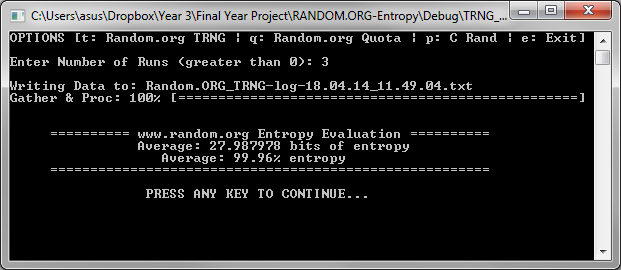
\includegraphics[scale = 0.75]{trng-ss.png}
\label{sngpss}
\end{figure}


\subsection{Conclusion}
This concludes the implementation phase of the project. I have now produced three working pieces of software; The Genetic Programming implementation of evolving RNGs, the Single Node Genetic Programming implementation and the implementation of the C RNG, and the random.org TRNG test. All of these implementations output data which shall be collected and used in the evaluation phase of this report.

While there were some hiccups during implementation as can be expected with the development of any piece of software, the process of creating and designing the algorithms and main methods in pseudo code in the design phase was of great use when it came to implementation. I was able to go relatively straight from pseudo code to C code which enabled me to finish all of the implementations a head of schedule (according to the gannt charts presented in all the documents).









































\newpage
\section{Evaluation}

\subsection{Introduction}
%- Introduce how evaluation is based on collecting data from running all implementations and then comparing the results. Any part where running time factors into the analysis then AMD Athlon X2 5600+ 2.8GHz Dual core processor used. Explain changes to the test criteria from design document.\\
The first phase of evaluation is to compare the results I obtained from implementing Koza's method of producing randomisers with the use of Genetic Programming. By looking at the data he obtained and what I obtained, we should be able to paint an accurate picture of how well I managed to convey his description in his paper \cite{kozarng}.

A major (arguably the most important) part of this project is to evaluate the results produced by both GP and SNGP implementations. The aim is to prove which method of genetically breeding RNGs produces the most solutions in the most efficient manner (with respect to running time and the size of the solutions produced). 50 runs were conducted for both the single threaded GP and SNGP implementations in order to compare averages of their outputs. Runs used for any part of the following analysis where run time is taken into consideration were ran on a machine with an AMD Athlon 64 X2 5600+ 2.8 GHz Dual-Core processor.

The next step of evaluation after that is to compare the RNGs produced by the GP and SNGP paradigms against two other RNGs in wide use today. The C $rand()$ function is a PRNG that uses a Linear Congruential Generator algorithm in order to give developers who are writing C programs a simple way of generating pseudo random numbers. The Hardware/True Random Number Generator at random.org collects binary data from a radio receiver that reads atmospheric noise produced by unpredictable natural effects such as lightning storms. There is an API available where developers can download ``true" random data from the random.org servers for use in their software\footnote{Please see the implementation section of this document for details on how this is achieved}. The randomness/entropy is tested in the same way for all approaches.

Sections of this evaluation have been changed and added since the design document was produced (please see the appendix for the original document). During implementation and initial evaluation, other ways of evaluating the project became apparent to me. I added the evaluation in section \ref{evalofgp} in order to assess how my results compared to the results presented by Koza in \cite{kozarng}. This way I can tell how accurately my implentation was to that proposed in the research paper. I also added the evaluation in section \ref{realimp}, which reviews how well the RNGs produced by Genetic means perform in a real software implementation. The reasoning behind this is that RNGs are frequently used by developers in various programming languages. I wanted to see whether it was practical for developers to use these RNGs produced Genetically in their software, again against the C $rand()$ function.

\subsection{Evaluation of GP Implementation}
%- Introduce evaluation by comparing first GP results to that of Kozas results. Compare any criteria that Koza proposes in his paper. Then show results and findings.\\
 \label{evalofgp}
The first stage of implementation as discussed in the Realistion seciton of this document was to follow Koza's Paper \cite{kozarng} in implementing a GP to evolve RNGs in C. To do this, I developed algorithms\footnote{Found in the Design section of this document and in the design document in the appendix} that expressed the processes, equations and design in his paper. The first part of the evaluation is to assess the results that Koza produced against what I managed to acheive from the carbon copy of his implementation.

In section 5.1 of \cite[p. 6]{kozarng}, Koza introduces his results from the run of the fittest solution produced by the GP implementation. In this run, Koza managed to produce a randomiser with an entropy of 27.996 bits on the 14th Generation. Koza describes the progression in fitness of the fittest candidate over these 14 generations. In order to make a comparison of one of my runs against Koza's run, I must also select the run that produced the fittest solution produced by my implementation. This run of mine took 10 generations to find a RNG with 27.995032 out of 28 bits of entropy.

Koza gives details of his run, saying; ``\emph{The best 24 individuals from generation 0 scored between 10.428 and 20.920 bits of entropy. The best single S-expression scored 20.920 bits.}". To compare this to my run, the best prefix expression\footnote{Koza wrote his implementation in LISP. S-Expressions and Prefix expressions are synonymous, as S-Expression are essentially prefix expressions with parenthesis} produced by generation 0 achieved 15.322 out of 28 bits of entropy.
Despite the lower fitness in generation 0, the progression of the fitness from therein was similar to that of Koza's run. After the description of generation zero, Koza goes onto explain; ``\emph{After 2 generations of one typical run, the entropy of the best-of-generation individual improved to 22.126 bits. After 4 generations, the entropy of the best-of generation individual improved to 26.474 bits. Thereafter, entropy reached and slowly improved within the 27.800 to 27.900 area.}". Again I obtained similar results from my run. After 2 generations the entropy of my best individual improved to 19.105 bits. After Generation 4 it had improved further to 21.005 bits. It improved gradually up until generation 8 where it took a leap from 24.295 to 27.915 bits. This was mainly down to the improvement of the 6 and 7 bit scalar entropies which jumped from 4.994 to 5.986 bits and 5.582 to 6.962 bits respectively between generations 7 and 8. The total entropy of the fittest candidate dropped slightly on generation 9 to 27.811 bits before finally rising to the terminating entropy of 27.995 bits on generation 10.

Koza also defined the scalar entropy breakdown of his fittest solution; ``\emph{In scoring 27.996, this randomiser achieved a maximal value of entropy of 1.000, 2.000, 3.000, 4.000, 5.000, and 6.000 bits for sequences of lengths 1, 2, 3, 4, 5, and 6, respectively, and a near-maximal value of 6.996 for the 128 (27) possible sequences of length 7.}" However, our fittest solution was not so uniform in breakdown. Instead it achieved maximal entropy of 1.000000 bits for sequences of length 1 and then 1.999935, 2.999866, 3.999688, 4.999333, 5.998764, 6.997446 bits for sequences of lengths 2, 3, 4, 5, 6, and 7 respectively. Therefore our solution here is slightly better at randomising sequences of length 7 bits, the same for length 1 bits, but slightly worse for 2, 3, 4, 5, 6 bits. Therefore it achieves a slightly lower overall entropy of 27.995 bits against Koza's 27.996 bits, but both remain highly credible randomisers with 99.98\% and 99.99\% entropy respectively. 

Coincidentally, the solution that I produced was not only the fittest but was also the quickest to find and had the smallest size over the 50 runs. It has only 15 points against Koza's 153 points, and as discussed above it took only 10 generations to find (434.4 sec). The prefix expression can be seen below;
\begin{center}
/\ -\ 2\ -\ 2\ J\ \%\ J\ -\ 2\ /\ /\ J\ 3\ 3
\end{center}
However the coincidence ends here. The average size of the solutions produced by our GP implementation is 154.6 points, very close to the 153 points in Koza's fittest candidate\footnote{Koza does not provide any average data or information for solution sizes.}
Here we have shown that using one run from both Koza's research in \cite{kozarng} and from the results that I have obtained by replicating his research, that the execution behaviour and the results are very similar.


\subsection{50 Standard Runs: GP vs SNGP Implementation}
%- Then introduce comparisons between GP and SNGP implementations under standard conditions for the 50 runs. Explain what will determine which method is most effective, i.e. minimal solution size, run time, highest fitness/entropy, highest solution rate, also average fitness of population increase of both. Then show results and findings and conclude to determine the victor.\\\
\label{gpvssngp}

In this section we compare the GP and SNGP implementations in order to uncover which is best suited for the problem domain of genetically breeding RNGs. In order to do this, data from 50 runs of both implementations were collected. These 50 runs were taken under standard conditions for both implementations as seen in the parameter definitions below in table \ref{standardparam}. For the GP implementation, these parameters were all taken from there definitions by Koza in \cite[p.6]{kozarng}. For the SNGP implementation, the termination fitness was also taken from Koza's definitions. The ``Mutation Attempts" and ``Population Size" parameters were taken as run conditions for SNGP defined by Jackson in \cite[p.54]{jacksonsngp}. %The Mutation Attempts has been ``manipulated to tune the solution rate, solution sizes, and speed of solution discovery.".

\begin{table}[H]
\caption{GP and SNGP Standard Parameters}
\centering
    \begin{tabular}{l|l|l}
    ~                                   & GP          & SNGP        \\ \hline
    Max Entropy                         & 27.990 Bits & 27.990 Bits \\
    Max Generations / Mutation attempts & 51          & 2500 \tablefootnote{Adaptation from 25000 to 2500 explained further on}        \\
    Population Size                     & 500         & 100         \\
    Max init program depth              & 4           & N/A         \\
    Max crossover program depth         & 15          & N/A         \\
    FPR prob                            & 0.1         & N/A         \\
    Crossover prob                      & 0.9         & N/A         \\
    Internal node crossover prob        & 0.9         & N/A         \\
    External node crossover prob        & 0.1         & N/A         \\
    \end{tabular}
\label{standardparam}

\end{table}

Now that we have defined the parameters, the data from 50 runs of the GP and SNGP implementations can be collected. The format of the data written by the runs can be found in section \ref{design}. The raw data written by the 50 runs can be found in the appendix, here this data shall be interpreted in order to conduct evaluation.

In order to correctly evaluate GP vs SNGP using this newly aquired data, we must first define the criteria which will determine the victor. The aim of any Genetic Program or Genetic Algorithm is to act as a search heuristic in order to find an optimal solution. Therefore like with any search algorithm, the desired characteristics are that it will produce a high rate of optimal solutions in an efficient manner. Applied directly to Evolutionary Algorithms, this corresponds to a process which produces the highest rate of short, highly fit solutions in the quickest time possible.

\subsubsection{Single Run Example}
Let's first introduce an example of a single run of both the SNGP and GP implementations that both managed to reach the termination entropy. In figure \ref{examplegrapha} below we can see already that in this instance SNGP has a more accelerated fitness progression and has a much shorter execution time;

\begin{figure}[H]
\centering
\label{examplegrapha}
\caption{Sample GP vs SNGP Run}
\resizebox{350pt}{!}{
\begin{tikzpicture}
\label{examplegrapha}
\begin{axis}[width=\textwidth, line width=2pt, font=\Large, grid=major,grid style={dashed}, cycle list name=androidstyle2, xmin = -50, xmax = 3500, ymin = 0, ymax = 30,
    xlabel={Time (Seconds)}, xtick={0,500,1000, 1500, 2000, 2500, 3000, 3500},
    ylabel={Entropy/Fitness (Bits)}]]
\addplot table [x=a, y=b, col sep=space, mark=none, smooth, color=dblue] {data.dat}  node[pos=1,pin={[pin distance=1cm]290:{\textbf{SNGP 624.6 Sec 27.99272 Bits}}}, inner sep=0pt, color=dblue] {};
\addplot table [x=c, y=d, col sep=space, mark=none, smooth, color=dred] {data.dat} node[pos=1,pin={[pin distance=2cm]265:{\textbf{GP 3399.6 Sec 27.99132 Bits}}}, inner sep=0pt] {};
\addplot [lblue, mark=x] coordinates {(624.599976, 27.99272)};
\addplot [lred, mark=x] coordinates {(3399.604004,27.99132)};
\addplot [dash pattern=on 1pt off 3pt] table [x = e, y = f,  col sep=space] {data.dat};

%\addplot [dash pattern=on 1pt off 3pt] table [x = g, y = h,  col sep=space] {data.dat};
\end{axis}
%\draw node [above] {};
%\draw node [label={[rectangle, draw=blue, thick, fill=blue!20, align=center, rounded corners, minimum height=2em, font=\tiny,label distance=3.3cm]40:Comparison of two successful, \\closest to average runs (with respect to run time)\\ of both SNGP and GP implementations.}] {};
\draw node [label={[label distance=12cm, font=\Large]80:Fitness threshold = 27.99 Bits of Entropy}] {};
\end{tikzpicture}
}
\label{examplegrapha}
\end{figure}

The fluctuation in entropy across the whole run is much less in SNGP than it is in GP. This is reflected when we show the scalar entropy breakdown for the same runs as seen below in figures \ref{sngpscalar} and \ref{gpscalar} below. We can see that the SNGP entropy rises in more uniform steps across all 1 - 7 bits, whereas GP fluctuates more aggressively. 
\begin{figure}[H]
\centering
\begin{minipage}{.5\textwidth}
  \centering
\captionof{figure}{Scalar Entropies SNGP}
\resizebox{220pt}{!}{
\begin{tikzpicture}
\begin{axis}[width=\textwidth, line width=1.2pt, xmin = 0, ymax = 8, font=\Large, cycle list name=androidstyle, grid=major,grid style={dashed},
    xlabel={Time (Seconds)},
    ylabel={Entropy/Fitness (Bits)}, ytick={1,2,3,4, 5, 6, 7},
legend style={
at={(-0.055,0.34)},
anchor=north east}]
\addplot table [x=a, y=b, col sep=space, mark=none, smooth, color=red] {data4.dat};
\addplot table [x=a, y=c, col sep=space, mark=none, smooth,  color=blue] {data4.dat};
\addplot table [x=a, y=d, col sep=space, mark=none, smooth,  color=green] {data4.dat};
\addplot table [x=a, y=e, col sep=space, mark=none, smooth,  color=red] {data4.dat};
\addplot table [x=a, y=f, col sep=space, mark=none, smooth] {data4.dat};
\addplot table [x=a, y=g, col sep=space, mark=none, smooth] {data4.dat};
\addplot table [x=a, y=h, col sep=space, mark=none, smooth] {data4.dat};
\end{axis}
\label{sngpscalar}
\end{tikzpicture}}
\end{minipage}%
\begin{minipage}{.5\textwidth}
  \centering
\captionof{figure}{Scalar Entropies GP}
  \resizebox{220pt}{!}{
\begin{tikzpicture}
\begin{axis}[width=\textwidth, xmin = 0, ymax = 8, line width=1.2pt, font=\Large, cycle list name=androidstyle, grid=major,grid style={dashed},
    xlabel={Time (Seconds)},
    ylabel={Entropy/Fitness (Bits)}, ytick={1,2,3,4, 5, 6, 7}, xtick={0,1000, 2000, 3000},
legend style={
at={(-0.055,0.01)},
anchor=north east}]

\addplot table [x=a, y=b, col sep=space, mark=none, smooth] {data5.dat};
\addplot table [x=a, y=c, col sep=space, mark=none, smooth] {data5.dat};
\addplot table [x=a, y=d, col sep=space, mark=none, smooth] {data5.dat};
\addplot table [x=a, y=e, col sep=space, mark=none, smooth] {data5.dat};
\addplot table [x=a, y=f, col sep=space, mark=none, smooth] {data5.dat};
\addplot table [x=a, y=g, col sep=space, mark=none, smooth] {data5.dat};
\addplot table [x=a, y=h, col sep=space, mark=none, smooth] {data5.dat};
\end{axis}
\label{gpscalar}
\end{tikzpicture}}
\end{minipage}
\end{figure}

\begin{figure}[H]
\centering
\hspace*{4em}
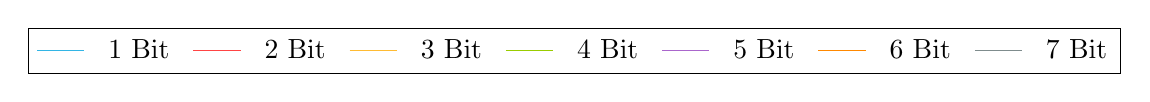
\begin{tikzpicture}
    \begin{customlegend}[legend columns=-1,legend style={column sep=1.5ex},legend entries={1 Bit, 2 Bit, 3 Bit, 4 Bit, 5 Bit, 6 Bit, 7 Bit}]
    \addlegendimage{lblue, sharp plot}
\addlegendimage{lred, sharp plot}
\addlegendimage{lorange, sharp plot}
\addlegendimage{lgreen, sharp plot}
\addlegendimage{lpurple, sharp plot}
\addlegendimage{dorange, sharp plot}
\addlegendimage{lgrey, sharp plot}
    \end{customlegend}
\end{tikzpicture}
\end{figure}
The reduced fluctuation for SNGP is down to the fact that it is driven by a hill climbing approach as discussed in both the design and implementation sections of this report. 
These two runs of each implementation were taken as closest to average for their running time with respect to the other 50 runs of each implementation. 

\subsubsection{50 Runs: Standard Parameters}
After 50 runs of both implementations under standard parameters, the following average results were achieved shown in table \ref{50average} below;

\begin{table}[H]
\caption{50 Run Average: GP vs SNGP}
\centering
    \begin{tabular}{l|l|l}
    ~                 & SNGP           & GP             \\ \hline
    Avg Run Time      &    \textcolor{red}{606.9s} &    4111.6s \\
    Avg Sol Run Time  & \textcolor{red}{483.2s}    & 2173.4s   \\
    Avg Non Sol Run Time  & \textcolor{red}{1701.1s}    & 5403.8s   \\
    Solution Rate     & \textcolor{red}{88\%}           & 40\%           \\
    Avg Sol Size\tablefootnote{\label{fixedsngpsize}Since the demonstration, solution size fixed for SNGP. It now corresponds to the number of nodes used in a solution.}  & \textcolor{red}{27.9} & 154.6          \\
    Avg Final Size\footnotemark[\ref{fixedsngpsize}]    & \textcolor{red}{30.1}        & 277.8          \\
    Avg Run Fitness   & \textcolor{red}{27.88153318}    &  27.2570626    \\
    Best Sol Fitness  & \textcolor{red}{27.995729}      & 27.995032      \\
    Avg Sol Fitness   & 27.9917378     & \textcolor{red}{27.99195145}    \\
    \end{tabular}
\label{50average}
\end{table}
SNGP comes out victorious on all tests bar the Average Solution Fitness (which is only beaten by 0.00076\% entropy). Over the 50 runs, SNGP finds over twice as many solutions, in under a quarter of the time. The solutions found are also on average 5 ${1} \over {2}$ times smaller due to the fact that branches in the trees are repeated (and can be calculated dynamically).

In \cite[p.54]{jacksonsngp} Jackson defines that the number of attempted $smut$ operations should be based on the number of individuals that would be processed in a traditional GP implementation. This is calculated by taking the product of the max number of generations\footnote{Not including the initial generation} and the size of the population. Therefore for our corresponding SNGP implementation this should be; $50*500 = 25000$. However Jackson also goes onto say in \cite[p.58]{jacksonsngp} ``\emph{these can be manipulated to tune the solution rate, solution sizes, and speed of solution discovery}". Therefore for the 50 runs I conducted for SNGP, I reduced the $smut$ attempts in order to show both a higher solution rate and a quicker running time. I did this by reducing the parameter from 25000 to 2500 attempts. Table \ref{25000} shows 10 runs with the $smut$ attempts set to 25000, and it shows that a 100\% solution rate can be achieved by doing so. However, taking a look back at our 50 runs, reducing this parameter by a $10^{th}$ did not reduce the solution rate by the same amount. In fact we can say therefore that on average 88\% of solutions are found within the first 2500 $smut$ attempts.

%Add fiugure mentioned above here.
\begin{table}[H]
\caption{10 Run Average: GP vs SNGP (25000 $smut$ limit)}
\centering
    \begin{tabular}{l|l|l}
    ~                 & SNGP           & GP             \\ \hline
    Avg Run Time      &    \textcolor{red}{1947.8s} &    4111.6s \\
    Avg Sol Run Time  & \textcolor{red}{1947.8s}    & 2173.4s   \\
    Solution Rate     & \textcolor{red}{100\%}           & 40\%           \\
    Avg Sol Size & \textcolor{red}{30.8} & 154.6          \\
    Avg Final Size  & \textcolor{red}{30.8}        & 277.8          \\
    Avg Run Fitness   & \textcolor{red}{ 27.99154673}    &  27.2570626    \\
    Best Sol Fitness  & \textcolor{red}{27.995936}      & 27.995032      \\
    Avg Sol Fitness   & 27.99154673    & \textcolor{red}{27.99195145}    \\
    \end{tabular}
\label{25000}
\end{table}

By increasing the number of $smut$ attempts from 2500 to 25000 we have obtained a 100\% solution rate but at the expense of having an average solution run time close to that of the GP average solution run time.

Therefore we can also say that using 2 independent runs (which can be run in parallel) of the SNGP paradigm given 2500 $smut$ attempts and given a success probability of $p_s = 0.88$, using simple probabilities, the chance of success over those two runs is equal to $1 - (1 - 0.88)^{2} = 0.9856$ or 98.56\%.  Therefore with a reduced $smut$ attempt parameter we can achieve a probability of success close to that of 100\%\footnote{Getting close but never quite 100\% due to the limit of the function ($\lim_{x \to \infty} 1 - (1 - 0.88)^{x} = 1$)} and benefit from a reduced amount of computation time.

By taking all 50 runs of each implementation (solutions and non-solutions), we can gain further insight into the relation between solution size, run time and entropy. To do this we can generate 3D surface plots from the data. In figures \ref{gpsurf} and \ref{sngpsurf} below we can see the correlation between solution size, fitness and run time for all 50 runs of both the GP and SNGP implementations respectively. As runs are independent to one another, so interpolation was required in order to create a surface in Matlab;

\begin{figure}[H]
\centering
\caption{GP surface plot}
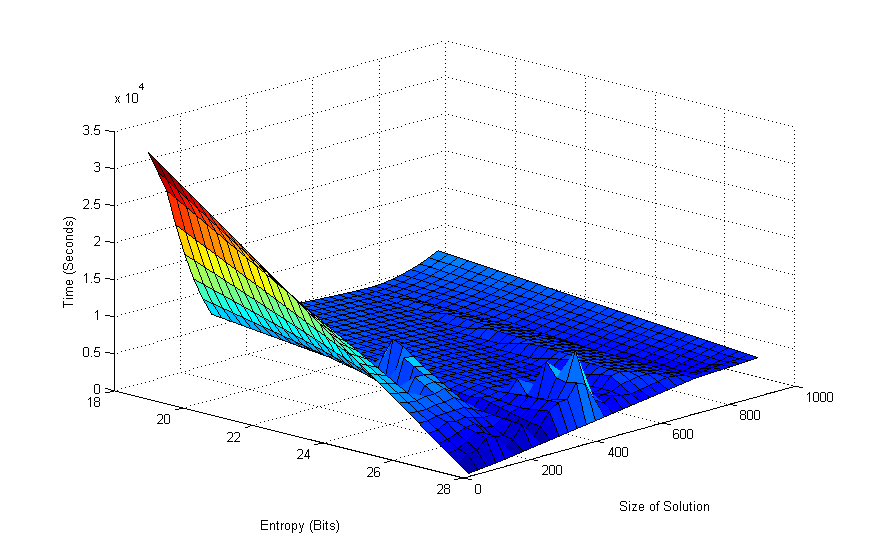
\includegraphics[scale = 0.6]{gp.png}
\label{gpsurf}
\end{figure}

In figure \ref{gpsurf} above we can see the correlation between  between solution size, fitness and run time for all 50 runs of the GP implementation. We can see that the scales are larger than that of the SNGP surface plot in figure \ref{sngpsurf} for solution size, fitness and run time. There is also less correlation between the runs/points on the plot compared to that of the SNGP plot. This reflects the lower solution rate that GP has, meaning that there aren't groups of points with high fitness plots like that evident in the SNGP plot below;

\begin{figure}[H]
\centering
\caption{SNGP surface plot}
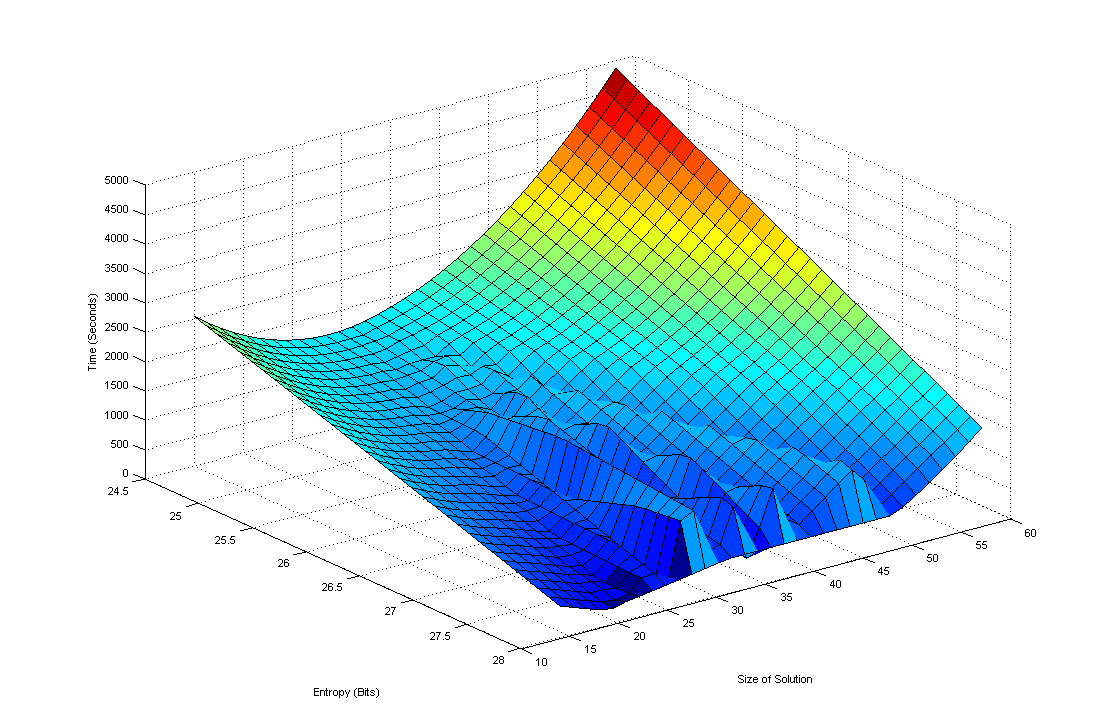
\includegraphics[scale=0.5]{sngp2.png}
\label{sngpsurf}
\end{figure}

\subsubsection{Fittest RNG Found}
After 50 executions of the SNGP and GP implementations, we were able to acheive a RNG with an entropy of 27.995729 out of 28 Bits in the SNGP implementation. The tree can be seen in figure \ref{fulltree} on page \pageref{fulltree} below.


\begin{sidewaysfigure}[!]
\caption{Fittest RNG Tree - 27.995729 Bits  of Entropy}
\label{fulltree}
\resizebox{750pt}{!}{
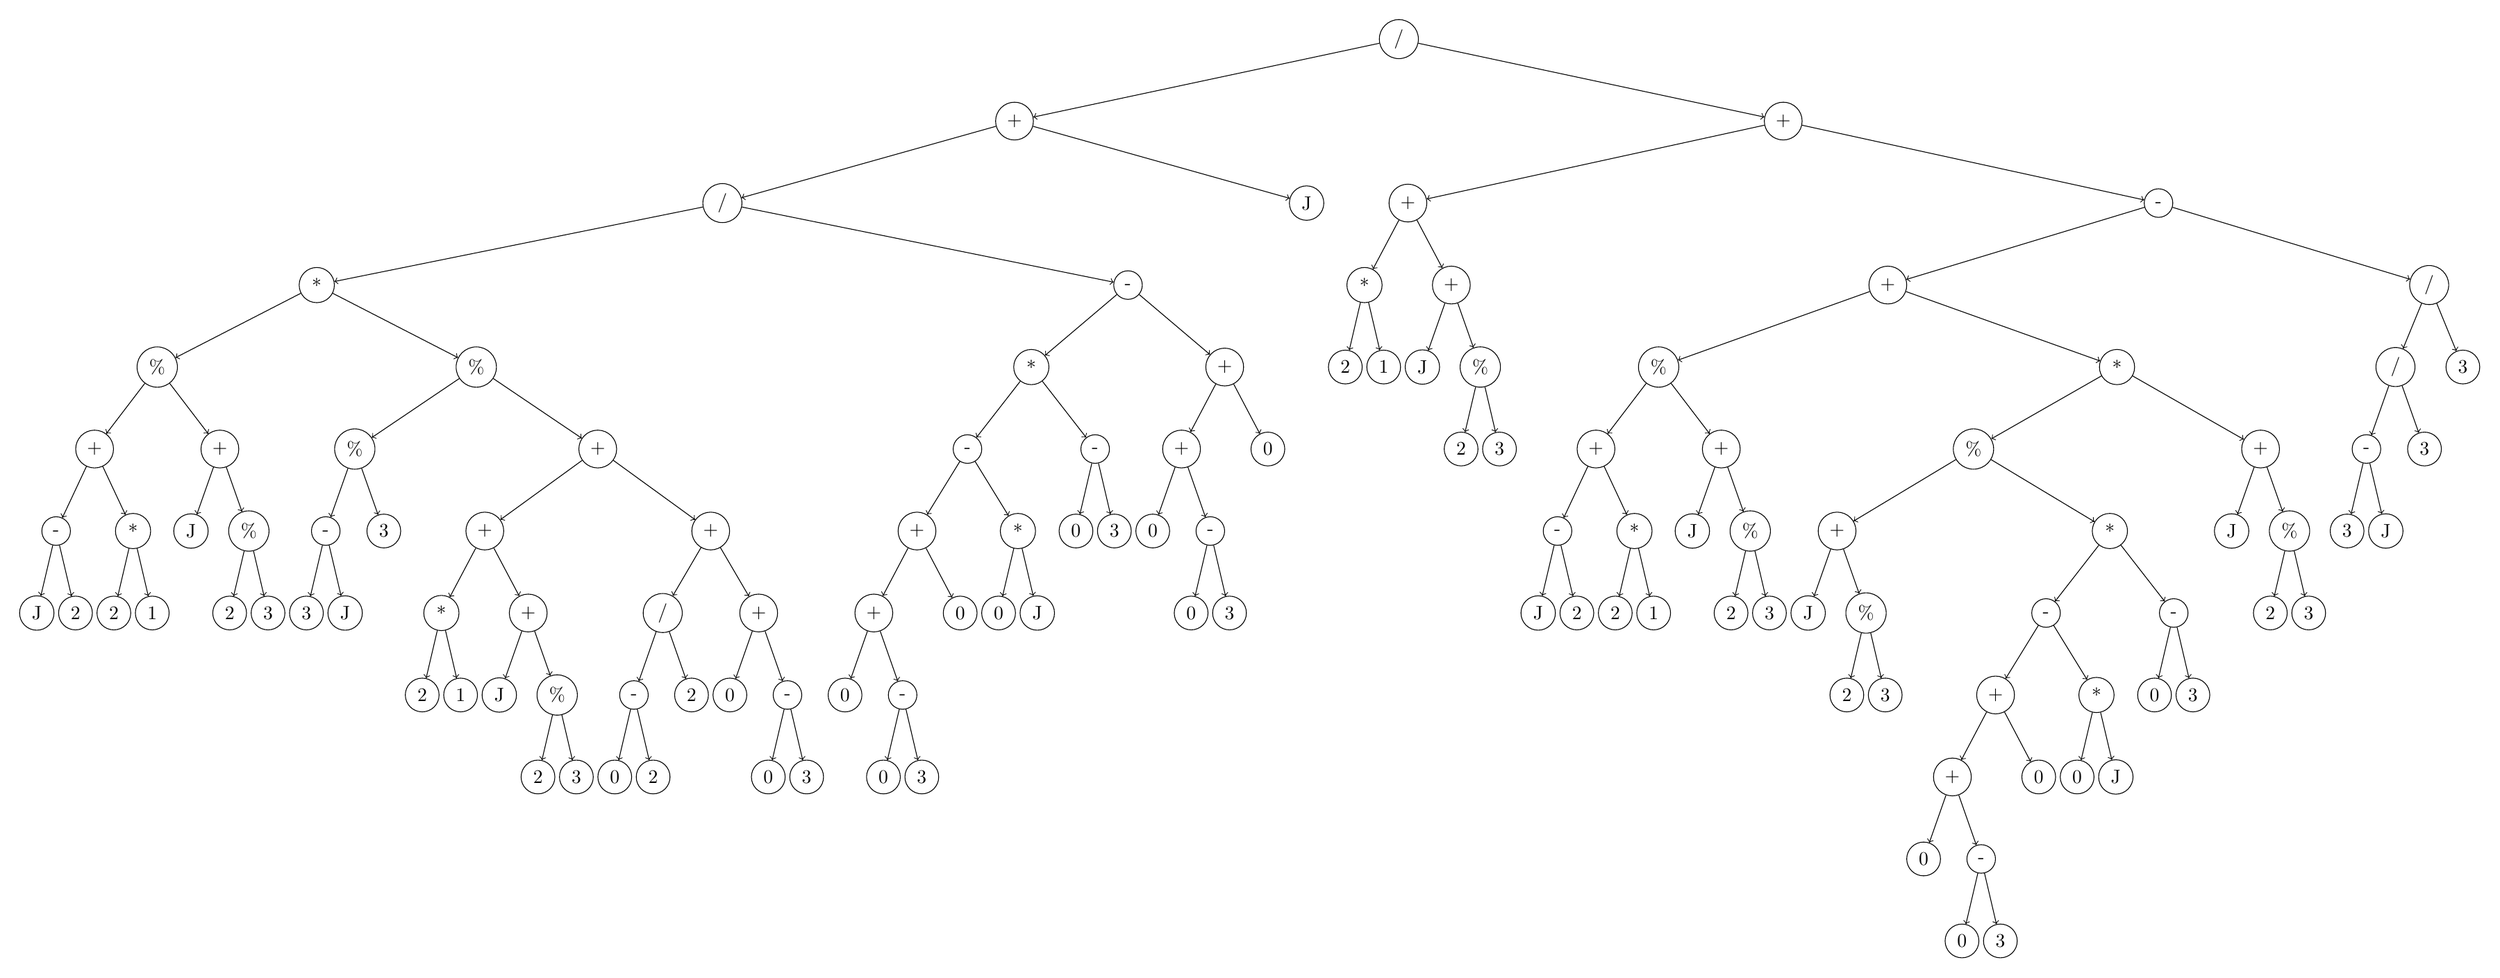
\begin{tikzpicture}[every tree node/.style={draw,circle,minimum size=1em}, level distance = 1.5cm,
edge from parent/.style={draw, ->, edge from parent path={(\tikzparentnode) -- (\tikzchildnode)}}]
\Tree[./ [.+ [./ [.* [.\% [.+ [.- J 2 ][.* 2 1 ]][.+ J [.\% 2 3 ]]][.\% [.\% [.- 3 J ]3 ][.+ [.+ [.* 2 1 ][.+ J [.\% 2 3 ]]][.+ [./ [.- 0 2 ]2 ][.+ 0 [.- 0 3 ]]]]]][.- [.* [.- [.+ [.+ 0 [.- 0 3 ]]0 ][.* 0 J ]][.- 0 3 ]][.+ [.+ 0 [.- 0 3 ]]0 ]]]J ][.+ [.+ [.* 2 1 ][.+ J [.\% 2 3 ]]][.- [.+ [.\% [.+ [.- J 2 ][.* 2 1 ]][.+ J [.\% 2 3 ]]][.* [.\% [.+ J [.\% 2 3 ]][.* [.- [.+ [.+ 0 [.- 0 3 ]]0 ][.* 0 J ]][.- 0 3 ]]][.+ J [.\% 2 3 ]]]][./ [./ [.- 3 J ]3 ]3 ]]]]
\end{tikzpicture}
}
\end{sidewaysfigure}

The RNG tree in figure \ref{fulltree} can be simplified by pre-calculating branches in the tree that operate only on constant values. When represented as an infix expression in a programming language, compliers will calculate this at compile time in order to reduce runtime in what's known as Constant Folding and Partial Redundancy Elimination. The tree in figure \ref{fulltree} can therefore be simplified into the tree in figure \ref{simplifiedtree} below.

\begin{figure}[H]

\centering
\caption{Simplified RNG Tree}
\resizebox{330pt}{!}{
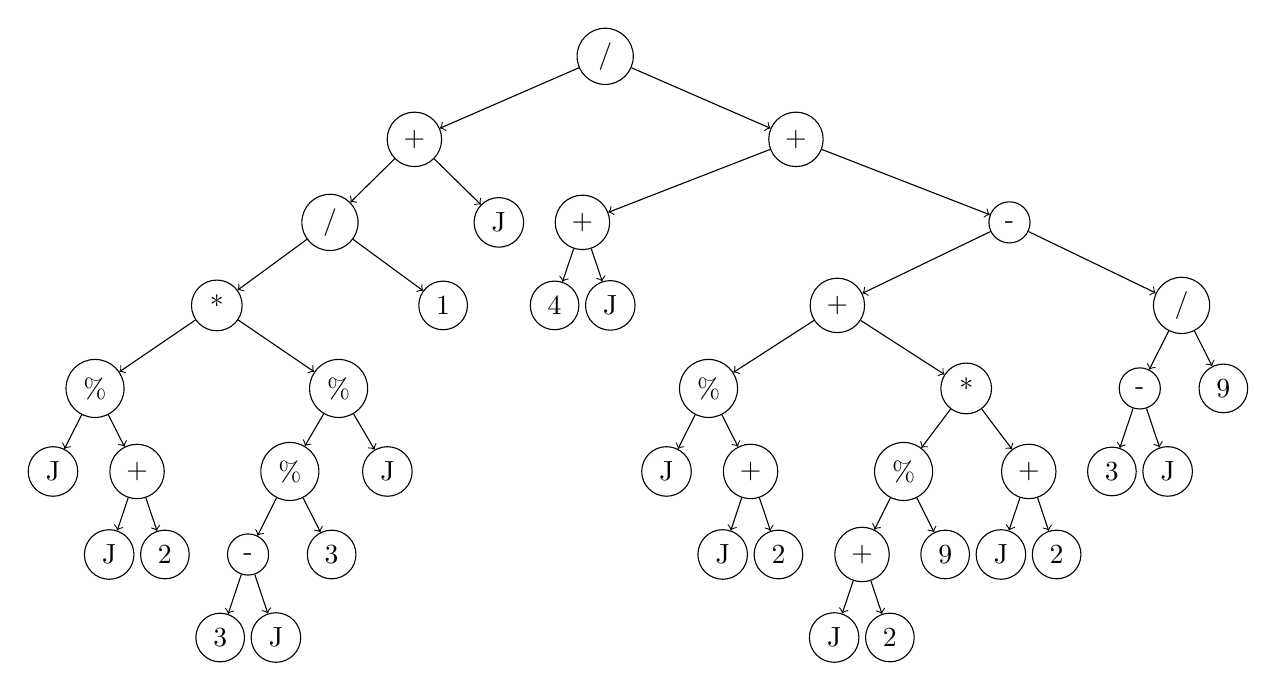
\begin{tikzpicture}[every tree node/.style={draw,circle,minimum size=1em},
edge from parent/.style={draw, ->,edge from parent path={(\tikzparentnode) -- (\tikzchildnode)}}]
\Tree[./ [.+ [./ [.* [.\% J [.+ J 2 ]][.\% [.\% [.- 3 J ]3 ]J ]]1 ]J ][.+ [.+ 4 J ][.- [.+ [.\% J [.+ J 2 ]][.* [.\% [.+ J 2 ]9 ][.+ J 2 ]]][./ [.- 3 J ]9 ]]]]
\end{tikzpicture}
}
\label{simplifiedtree}
\end{figure}
This simplified tree can be represented as an infix mathematical function $f(J)$ below;
\begin{equation*}
f(J) = {{\left( (J\bmod (J+2))\ *\ (((3-J)\bmod 3)\bmod J) \over 12 \right) + J} \over {(4 + J) + \left((J\bmod(J+2) + ((J+2)\bmod 9) * (J+2)) - ({3-J \over 9}) \right)}}
\end{equation*}
Such an infix expression can be implemented into a program (i.e. into code). This shall be discussed later in the report.
\subsubsection{GP vs SNGP Conclusion}
We can conclude that for the purposes of producing RNGs by genetic means, that SNGP is a substantially more efficient and more successful paradigm to implement to solve the problem than GP is. We have also shown that it is possible to manipulate the number of $smut$ attempts (increase it 10 fold) to achieve a 100\% solution rate.

\newpage
\subsection{Parameter Altering Experimentation: Reducing Population Sizes}
In this section we take a look at the effects of altering the population size of the GP and SNGP implementations, in order to see what effect different conditions have on their performance. On \cite[p.56]{jacksonsngp} Jackson experiments with the effects of reducing the population size on the solution rate of his 6-mux SNGP implementation. In section \ref{gpvssngp} we take a look at increasing the number $smut$ attempts on the performance of the SNGP model. In figures \ref{sngpreduceda} and \ref{gpreduceda} below we can see the effects of a reduced population on the rate of solutions produced by both methodologies. For SNGP I gathered data from 10 runs at each of the following 20\% population size decrements (and a final 10\% decrement) \{100, 80, 60, 40, 20, 10\}. I gathered the same data from the GP implementation for the populaiton size decrements of \{500, 400, 300, 200, 100, 50\}. The results I obtained can be seen below;


\begin{figure}[H]
\centering
\begin{minipage}{.5\textwidth}
  \centering

\captionof{figure}{Reduced Pop size of SNGP}
\resizebox{220pt}{!}{
\begin{tikzpicture}
\begin{axis}[width=\textwidth, line width=2pt, grid=major,grid style={dashed}, ymax = 100, ymin = 0, xmin = 0, xmax = 100, every axis label/.append style={font=\Large}, every tick label/.append style={font=\Large},
    xlabel={Population Size},
    ylabel={Solution Rate (\%)}, smooth,  xtick={0,20,40,60, 80, 100},
stack plots=y,
enlarge x limits=false]
\addplot [color=lblue] table [x=a, y=b, col sep=space, mark=none, smooth, color=lblue] {sngpreduced.dat}  {};
\end{axis}
\end{tikzpicture}}
\label{sngpreduceda}
\end{minipage}%
\begin{minipage}{.5\textwidth}
  \centering

\captionof{figure}{Reduced Pop size of GP}
  \resizebox{220pt}{!}{
\begin{tikzpicture}
\begin{axis}[width=\textwidth, line width=2pt, grid=major,grid style={dashed}, ymax = 100, ymin = 0, xmin = 0, xmax = 500, every axis label/.append style={font=\Large}, every tick label/.append style={font=\Large},
    xlabel={Population Size},
    ylabel={Solution Rate (\%)}, smooth,  xtick={0,100,200,300,400, 500},
stack plots=y,
enlarge x limits=false,]
\addplot [color=lred] table [x=a, y=b, col sep=space, mark=none, smooth, lred] {gpreduced.dat}  {};
\end{axis}
\end{tikzpicture}}
\label{gpreduceda}
\end{minipage}

\end{figure}

It seems that for both implementations, the solution rate stays relatively the same (bar the 20\% anomaly for size 300 in GP) until after the population size is set lower than the average size of solutions for the 50 runs as discussed earlier. For GP the average size of solutions 156.4 and the solution rate becomes 0\% after the population size is set to less than or equal to 100. For SNGP the average size of solutions is 27.9, and the solution rate for SNGP is reduced to 0\% when the population size is set less than or equal to 10.

In figures \ref{sngprun} and \ref{gprun} below, we can also see the reduction in average running time of both the SNGP and GP implementations when the population size is lowered respectively;


\begin{figure}[H]
\centering
\begin{minipage}{.5\textwidth}
  \centering

\captionof{figure}{Avg SNGP Run Time with Reduced Pop}
\resizebox{220pt}{!}{
\begin{tikzpicture}
\begin{axis}[width=\textwidth, line width=2pt, grid=major,grid style={dashed}, ymax = 900, ymin = 0, xmin = 0, xmax = 100, every axis label/.append style={font=\Large}, every tick label/.append style={font=\Large},
    xlabel={Population Size},
    ylabel={Time (Sec)}, smooth,  xtick={0,20,40,60, 80, 100},
stack plots=y,
enlarge x limits=false]
\addplot [color=lblue] table [x=a, y=b, col sep=space, mark=none, smooth, color=lblue] {sngpreducedrun.dat}  {};
\end{axis}
\end{tikzpicture}}
\label{sngprun}
\end{minipage}%
\begin{minipage}{.5\textwidth}
  \centering
\captionof{figure}{Avg GP Run Time with Reduced Pop}
  \resizebox{220pt}{!}{
\begin{tikzpicture}
\begin{axis}[width=\textwidth, line width=2pt, grid=major,grid style={dashed}, ymax = 4200, ymin = 0, xmin = 0, xmax = 500, every axis label/.append style={font=\Large}, y tick label/.append style={font=\large}, x tick label/.append style={font=\Large},
    xlabel={Population Size},
    ylabel={Time (Sec)}, smooth,  xtick={0,100,200,300,400, 500},
stack plots=y,
enlarge x limits=false,]
\addplot [color=lred] table [x=a, y=b, col sep=space, mark=none, smooth, lred] {gpreducedrun.dat}  {};
\end{axis}
\end{tikzpicture}}
\label{gprun}
\end{minipage}
\end{figure}

In figure \ref{gprun} above we see the expected reduction in run time as we reduce the population size. This is because the number of individuals being processed is being reduced and therefore the number of trees that must be evaluated and tested for fitness is also reduced. However in figure \ref{sngprun} above we see that the average computation time actually rises from 606 to 868 seconds when the population size is reduced from 100 to 80, and doesn't actually drop back below 606 seconds until a population of size 40. This can be seen as an anomaly (as only 10 runs were taken for each population size). However it could be reasoned that we know (from our 50 runs in figure \ref{50average} on page \pageref{50average}) that runs that fail to find a solution take on average 3.5 ($1701.1 / 483.2 = 3.521$) times longer to find a terminate than those that do. Therefore if the solution rate drops from 88\% to 80\%, this will have a knock on effect to the average running time for not finding solutions (minus the reduced running time for processing less individuals). For instance, when the solution rate levels off at 60\% between 40 and 20 the run time decreases, as a reduced population size with the same solution rate will definitely incur a reduced run time.

Here we have shown that a reduced population size can reduce the run time both implementations whilst still yielding an acceptable solution rate. However we have also shown that (in the case of SNGP) a reduced population size that reduces the solution rate can lead to non solution times having a more aggressive effect on the average run time than the reduction in time that having less individuals to process does.

\subsection{Genetic vs Conventional RNGs}

Now that we have determined that SNGP is substantially better suited for the actual process of generating of RNGs, we can now use the RNGs in order to compare them against other conventional RNGs. As discussed earlier in this report, I have chosen two different random number generators as competitors to our genetically bred solutions. I chose the C $rand()$ function incorporated in the standard C programming language library as a comparable PRNG that (like our RNGs) produces numbers deterministically. Unlike our RNGs which use a sequence of integers, the C $rand()$ function uses a Linear Congruential Generator (LCG) algorithm which uses a seed value in it's equation in order to output a number which is then used as the seed for the next call. This LCG algorithm/equation can be seen below;

\begin{center}
\noindent\begin{minipage}{.5\linewidth}
\begin{equation*}
X_{n+1} = (aX_n + c)\mod m
\end{equation*}
\end{minipage}%
\begin{minipage}{.4\linewidth}
where;\\
$m, 0 < m$ - the modulus\\
$a, 0 < a < m$ - the multiplier\\
$c, 0 \leq c < m$ - the increment\\
$X_0, 0 \leq X_0 < m$ - the seed
\end{minipage}
\end{center}

As shown in \cite{lcghack}, LCGs are vulnerable to attack. In the paper it is shown that the variable $m$ in the equation above can be calculated given only 3 outputs due to how LCG outputs commonly fall into 3 dimensional planes. A possibility with using RNGs that are evolved genetically, is that their formula would not be widely known and the formula itself can be updated periodically by the implementer by generating new RNGs.

For the other comparable RNG, I chose a Hardware / True Random Number Generator. This way we can compare our genetically bred randomisers to a source of non-deterministic random data (i.e. the random values are not the result of some deterministic algorithm or equation). I chose to specifically use the service provided at random.org, where their servers provide random binary digits generated from observed atmospheric noise on demand. 

We analyse the random data produced by these two methods in the same way as our fitness function in our Genetically bred RNGs. Using the Shannon entropy equation we can gather 16834 bits from the other two RNGs and calculate the entropy for binary subsequences of lengths 1 to 7 bits. This way we can test all of our RNGs fairly under the same conditions and using the same test.

I used the data from the 50 runs of our GP and SNGP implementations, and then ran the same number of tests on the conventional RNGs. The results can be seen in table \ref{allrandomresult} below;


\begin{table}[H]
\centering
\caption{TRNG vs C PRNG vs SNGP vs GP}
\label{allrandomresult}
    \begin{tabular}{l|l|l|l|l}
    ~                     & TRNG\tablefootnote{Fixed since demonstration (The test code was including some formatting characters and not just binary data)}           & C PRNG         & SNGP           & GP             \\ \hline
    Fittest (Entropy)               &    27.993975   &    27.991925   &    \textcolor{red}{27.995729}   &    27.995032   \\ \hline
    Fittest (\%)               &    99.978\%  &    99.971\%  &    \textcolor{red}{99.985\%}   &    99.982\%  \\ \hline
    Fittest (Entropy Shortfall)               &    0.006025   &    0.008075  &    \textcolor{red}{0.004271}   &    0.004968   \\ \hline
    Avg Fit (Entropy) (Sol) &    27.98997218 &    27.98985372 &    27.9917378  &    \textcolor{red}{27.99195145} \\ \hline
   Avg Fit (\%) (Sol) &    99.9641\% &    99.9637\% &   99.970\%  &    \textcolor{red}{99.971\%} \\ \hline
   Avg Fit (Shortfall) (Sol) &    0.01002782 &   0.01014628 &    0.0082622  &    \textcolor{red}{0.00804855} \\ 
    \end{tabular}
\end{table}

From the results shown above we can see that the RNGs produced by Genetic means outperform both the C $rand()$ function and the TRNG in terms of entropy. SNGP produces the candidate with the highest fitness and GP produces the highest average fitness (slightly higher than that of SNGP which also beats the two conventional methods). Whilst the genetic RNGs only beat the conventional methods by a fraction, this small improvement can make all the difference when producing high entropy random digits.

The C $rand()$ function performs the worst out of all four candidates producing both the lowest best run and the lowest average fitness (albeit very marginally to the TRNG). The TRNG then places $3^{rd}$ producing lower average fitness and lower best run fitness than both of our evolutionary methods.

Random data can be interpreted in different mediums such as in audio, video and images. We can create 128x128 ($\sqrt{16384} = 128$) images for each of our random methods by interpreting a single bit as a black pixel if it is equal to 1 or as a white pixel if it is equal to 0 from the sequence of 16834 bits. 

The images in figures \ref{cpica}, \ref{trngpica} and \ref{geneticpica} were created from 3 runs chosen from each of the methods;
\begin{figure}[H]
%\centering
\begin{minipage}{.35\textwidth}

\caption{C $rand()$ Image}

\includegraphics[keepaspectratio=true, height= 150pt]{crand.png}
\label{cpica}
\end{minipage}%
\begin{minipage}{.35\textwidth}

\caption{Random.org Image}

\includegraphics[keepaspectratio=true, height= 150pt]{randomorg.png}
\label{trngpica}
\end{minipage}%
\begin{minipage}{.35\textwidth}

\caption{Genetic Image}

\includegraphics[keepaspectratio=true, height= 150pt]{myrand.png}
\label{geneticpica}
\end{minipage}%
\end{figure}

As we can see the C $rand()$ function displays repetitions at uniform intervals giving rise to verticall patterns (the images are populated with pixels from to left to top right and then repeated down the image) . This shows that numbers are repeated more often as well giving it a lower entropy. The data from random.org has no distinguishable patterns at all, however this does not necessarily correspond to a higher entropy, as numbers may still be repeated just not in a uniform fashion like that of the C $rand()$ function. On close inspection the data / image from the genetic RNG might show a subtle pattern to some viewers eyes. This is in fact what gives rise to its very high entropy; a uniformity in distribution and a lower repetition. As our genetic RNG has the highest entropy, in these 16384 bits/pixels (128x128) every binary subsequence of length 1 to 7 needs to occur with (almost) equal probability. Therefore when the GP and SNGP are genetically "engineering" this through evolution, it causes RNGs to produce some uniformity.

Below is a graph produced by the random.org servers displaying the shortfall in entropy on the same day on which I collected my test data. As the website provides no specific details on the size and length of bit sequences on which the output from their TRNG is tested, the use of this graph isn't a fair comparison against our other RNGs. However it seems that the average is around 99.96\% to 99.7\% which is close to the results we obtained. As we can see from the graph, as the source of the TRNG is non deterministic, the entropy can fluctuate quite aggressively;

\begin{figure}[H]
\label{trngpic}
\centering
\caption{Random.org Entropy Shortfall}
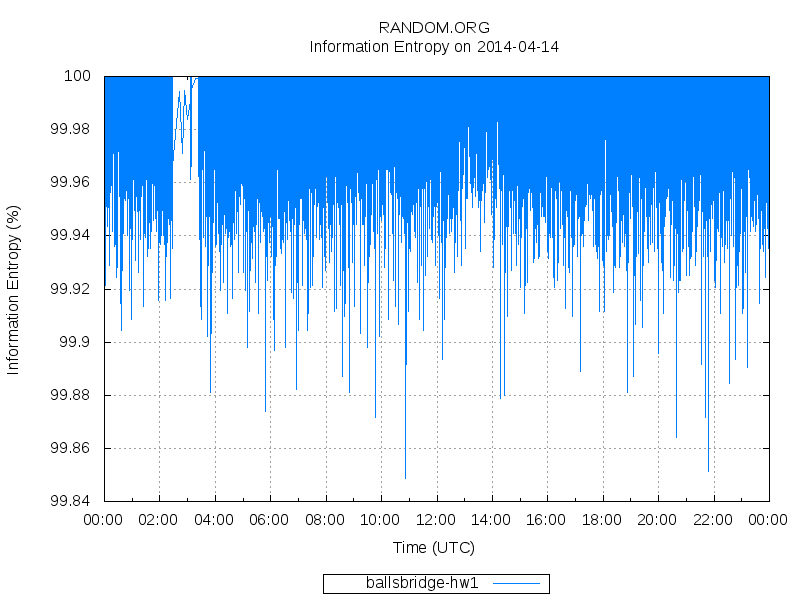
\includegraphics[keepaspectratio=true, height= 280pt]{trng.png}
\end{figure}
 
For comparison, the shortfall in entropy of SNGP and GP solutions can be seen in figures \ref{sngpshort} and \ref{gpshort} below.
\begin{figure}[H]
\centering
\begin{minipage}{.5\textwidth}
  \centering

\captionof{figure}{SNGP Entropy Shortfall of Solutions}
\resizebox{220pt}{!}{
\begin{tikzpicture}
\begin{axis}[x=8pt, width=\textwidth, line width=0pt, font=\Large, bar width=3pt, axis on top, ymax=100, ymin=99.96, grid=major,grid style={dashed}, xmin = 1, xmax = 45,  line width=1.5pt, smooth,
stack plots=y,  y label style={at={(axis description cs:-0.01,.5)},anchor=south},
area style,
enlarge x limits=false,
    xlabel={Run Number},
    ylabel={Entropy (\%)}]]

\addplot [lblue] table [x= a, y=c] {data2.dat};    % Plot the "First" column against the data index

\end{axis}
\end{tikzpicture}}
\label{sngpshort}
\end{minipage}%
\begin{minipage}{.5\textwidth}
  \centering
\captionof{figure}{GP Entropy Shortfall of Solutions}
  \resizebox{220pt}{!}{
\begin{tikzpicture}
\begin{axis}[x=18pt, width=\textwidth, line width=0pt, font=\Large, bar width=8pt, axis on top, ymin=99.96, grid=major, grid style={dashed}, xmin = 1, xmax =20,ymax=100, line width=1.5pt, smooth,
stack plots=y,
area style,  y label style={at={(axis description cs:-0.01,.5)},anchor=south},
enlarge x limits=false,
    xlabel={Run Number},
    ylabel={Entropy (\%)}]]

\addplot [lred] table [x= a, y=b] {data3.dat};  

\end{axis}
\end{tikzpicture}
}
\label{gpshort}
\end{minipage}
\end{figure}


To conclude, statistically the RNGs produced by evolutionary means outperform the two common conventional methods as far as we are concerned with entropy. To someone else however the data in the image produced by the TRNG may be deemed more ``trustworthy" or more random due to its non-uniformity in distribution. As far as PRNGs go however, both visually and statistically our RNGs produced by evolutionary means are evidently superior to the C $rand()$ function. 

\subsection{Real Implementation}
 \label{realimp}
Now that we have shown the RNGs produced by genetic means are superior (in terms of entropy) to widely used conventional methods of producing random numbers, another way to assess the successfulness of this project is to see their real world application. Take the fittest and smallest solution produced by the GP implementation as discussed in section 5.2;

\begin{center}
/\ -\ 2\ -\ 2\ J\ \%\ J\ -\ 2\ /\ /\ J\ 3\ 3
\end{center}
This RNG achieved 27.995032 out of 28 bits of entropy. It can be represented as an infix mathematical function like so;

\begin{equation*}
rand(J) = {{(2 - ( 2 - J))} \over {J \mod (2 - \left({J \over 6}\right))}}
\end{equation*}
Remember that as discussed before, the RNGs are evolved on their binary output entropy and not as integer interpretation. Therefore in order to obtain integers with high entropy in an implementation, the RNG must create a stream of binary digits to then be interpreted as integers. They are also evolved based on their ability to randomise a sequence and not as a LCG. Therefore, in an implementation a seed value should be attained and then incremented in order to produce the best results. An example implementation of the function above can then be implemented in C code as seen below. 
\begin{lstlisting}[language=C, basicstyle=\small]
int randomiser(int min, int max) {
	max++; //Incrementing Max as to include it as a possible random output.
	int dec = 0;
	//Taking into account a negative minimum
	if (min < 0)
		max = (-1*min) + max;
	//Calculating the length of the stream we need
	int bit_max = (int) ceil(log10((double)max)/log10((double)2)); 
	//For that length we can read in the binary output of the random number generator
	for (int i = 0; i < bit_max; i++) {
		if ((protected_div(2 - (2 - seed), protected_mod(seed, (2 - (protected_div(protected_div(seed, 3), 3))))) % 2) == 1)
			dec = dec + pow((double)2, i);
		seed++; //Running through the sequence as we do.
	}
	//Returning the value between the defined range, taking into account a negative min
	int rand_return = 0;
	if (min < 0)
		rand_return = (dec % max) - (-1*min);
	else
		rand_return = ((dec % (max-min)) + min);
	return rand_return;
}
\end{lstlisting}
As discussed earlier the protected division and protected modulo functions return 1 if division or modulo by 0 is attempted.
This function can be seeded and called like so;

\begin{lstlisting}[language=C, basicstyle=\small]
int seed = time(NULL); //Seeded with the current time
int rand = randomiser(-300, 2000); //Generate a random number between -300 and 2000
\end{lstlisting}
Calling the randomiser function 100 times using the same parameters as seen above gave the following output;

\begin{lstlisting}[language=C, basicstyle=\small]
637  886  136  605  1256 393  555  213  969  715  290  1813 1429 557  26   1317 
1369 1441 157  -169 1668 689  -8   1028 429  1106 24   665  847  160  940  -144
-237 -215 1138 -235 286  1007 -86  1266 -225 1111 1518 -62  1023 984  1218 1235
1881 1788 1201 1903 -294 1244 1375 1258 380  1624 167  440  -141 1956 557  -273
778  495  1047 1288 706  1323 1908 1594 1076 665  1261 31   1432 1397 166  279
975  1195 1758 1084 932  658  84   408  400  168  420  337  72   -222 561  -122
485  -16  -154 792

\end{lstlisting}
Using this method, while producing a higher entropy result, is computationally more intensive than the C rand() function. This is because the RNG must be called $n$ times where $n$ is the number of bits required to reach the $max$ value defined by the user. This RNG can easily be parallelised however, so each RNG call can be done in parallel (because we can predict the seed values in advance). As we can see in figure \ref{rngcalls}, the running time of both the C rand() function and our genetically evolved RNG with respect to the number of calls on both are of the same order. However there exists some constant number of operations in our RNG implementation, that causes a longer over all running time. We can also see in figure \ref{rngmax} that over 1000 runs of each input, a higher value has no effect on the c rand() function, as the limit of the number is done with a simple modulus function. With our implementation of the genetically bred RNG, the max input size dictates how many bits we need and therefore how many calls of the RNG we need. Hence a larger max value has an effect on the running time (albeit small). We can conclude therefore that if an implementation of our RNG was desired by a developer, then a higher entropy output would come at the expense of computation time.

\begin{figure}[H]
\centering
\captionof{figure}{Logarithmic (base 10) Scale Run time of $n$ calls of $rand(J) = {{(2 - ( 2 - J))} \over {J \mod (2 - \left({J \over 6}\right))}}$ and C $rand()$, on the fixed min value of 0 and max value of 2000 for all runs}
\resizebox{350pt}{!}{
\begin{tikzpicture}
\label{rngcalls}
\begin{axis}[width=\textwidth, line width=2pt, grid=major,grid style={dashed}, ymax = 240, xmax = 10000000000, every axis label/.append style={font=\Large}, every tick label/.append style={font=\Large},
    xlabel={Number of Calls (n)},
    ylabel={Run Time (sec)}, smooth, xmode=log,
       log basis x={10}, legend style={
at={(0.55,0.34)},
anchor=north east},
enlarge x limits=false]
\addplot [color=lgreen] table [x=a, y=b, col sep=space, mark=none, smooth, color=lblue] {cvsmyrand.dat}  {};
\addplot [color=lorange] table [x=a, y=b, col sep=space, mark=none, smooth, color=lblue] {cvsmyrandc.dat}  {};

\legend{$rand(J) = {{(2 - ( 2 - J))} \over {J \mod (2 - \left({J \over 6}\right))}}$,C $rand()$}
\end{axis}
\end{tikzpicture}}
\end{figure}

\begin{figure}[H]
\centering
\captionof{figure}{Effect of increasing max value of random number on run time, 1000 calls for each max value. Logarithmic (base 10) Scale Run time of $rand(J) = {{(2 - ( 2 - J))} \over {J \mod (2 - \left({J \over 6}\right))}}$ and C $rand()$}
\resizebox{350pt}{!}{
\begin{tikzpicture}
\label{rngmax}
\begin{axis}[scaled ticks=false, tick label style={/pgf/number format/fixed}, width=\textwidth, line width=2pt, grid=major,grid style={dashed}, xmax = 10000000, every axis label/.append style={font=\Large}, every tick label/.append style={font=\Large},
    xlabel={Max value (n)},
    ylabel={Run Time (sec)}, smooth, xmode=log, ytick={0.00, 0.01,0.02,0.03,0.04,0.05,0.06},
       log basis x={10}, legend style={
at={(0.60,0.33)},
anchor=north east},
enlarge x limits=false]
\addplot [color=lgreen] table [x=a, y=b, col sep=space, mark=none, smooth, color=lblue] {rand_runtime.dat}  {};
\addplot [color=lorange] table [x=a, y=c, col sep=space, mark=none, smooth, color=lblue] {rand_runtime.dat}  {};

\legend{$rand(J) = {{(2 - ( 2 - J))} \over {J \mod (2 - \left({J \over 6}\right))}}$,C $rand()$}
\end{axis}
\end{tikzpicture}}
\end{figure}


\newpage

\section{Discussion}
\label{discussion}
Having completed this project, I leave open further research that can be conducted. A multi objective optimisation implementation for GP and SNGP may be implemented in order to produce RNGs which are not only capable of producing high entropy, but also perform well in other statistical tests for randomness covered in the NIST test suite \cite{nist}. Of course, there would most likely be some amount of trade off between multiple statistical results, so the termination entropy may need to be lowered in order to obtain results. 

Further mathematical operators could be added to the set of functions. By taking $x$ as the value of the left branch and $y$ the value of the right branch, any mathematical operation with an arity of two might be used. This could include the exponent function ($x^y$ - although this is a computationally intensive function) or the logarithmic function (with either a coefficient and a static base i.e. $x \log_2 y$, or a dynamic logarithmic variables i.e. $\log_x y$). The $x^{th}$ root function could also be used, in the form $\sqrt[x]{y}$ where again, $x$ and $y$ are the values of the two branches of the node.

These operations may lead to larger computation times against the simple mathematic operators used in this project, but they may also lead to fitter solutions.

\section{Learning Points}
In Summer 2013 after selecting this project I began doing preliminary reading around the areas of Genetic Algorithms and Genetic Programming. Before this time, I had read only briefly around what GP and GAs were capable of solving and their basic structure. I chose this project for two reasons; one because I thought that this was a very interesting application of Genetic Programming, and the second as I wanted to further broaden my knowledge in the area of Computer Science instead of doing a project on something I already had a lot of prior knowledge of. Therefore this project has not only been a success in proving that SNGP is a more effective method for evolving RNGs and Genetic RNGs can perform better than other widely used RNGs, but it has also been a great success in educating me in an area which I also wish to continue to do further research in.

Initially I began reading around the area of Genetic Algorithms, crucially using the book ``An Introduction to Genetic Algorithms" by Melaine Mitchell \cite{mitchell}, which gave me a solid introduction into the world of evolutionary computation. I then refined my reading towards Genetic Programming. Whilst \cite{mitchell} covers Genetic Programming breifly in the book, I moved onto a more detailed and focused book entitled ``Genetic Programming. On the Programming of Computers by Means of Natural Selection" by John Koza \cite{kozagpbook}. John Koza is a pioneer of Genetic Programming, and his work on evolving RNGs using Genetic Programming in \cite{kozarng} was the basis for this project (along with Jacksons research on SNGP). From all of this reading and research I gained a solid understanding of the area of Evolutionary Computing and more specifically Genetic Programming.

% Extensive design is useful
Having written all of the main algorithms and pseudo-code for the GP and SNGP models in the design section, the process of implementation went much smoother than I had first expected. I spent the majority of the time during implementation simply translating the algorithms from pseuod-code to C code. There were fewer bugs and semantic errors than I had anticipated, and as a result I was able to finish implementation ahead of schedule. From this process I was able to learn that thorough design can save a lot of time during implementation. From past projects (academic and non-academic) where design was not as extensive I had spent longer in the implementation stage. In the future for any projects and research I conduct, I now know that a through design can save me time and make implementation simpler to translate from design to code.

%improved research techniques and analysis of data
This project has also further improved my skills in research. My ability to use scientific papers related to the work I am conducting in order to further build upon and find new ways of comparing results has vastly improved in the duration of this project. A large section of this project was down to analysing and evaluating the performances of all methods of producing random numbers. My analysis techniques have also been improved during this project, I have developed better approaches to testing thoroughly and well and hope to carry what I have learnt into research projects in the future. 


%%Gaining a mathematical of Information theory (Entropy), Improved programming abilities and better C development. Improved LaTeX skills, useful for further research and paper writing.
From a technical standpoint, I now have a better mathematical understanding of information theory and entropy, and also improved C programming abilities especially when implementing the Shannon entropy equation in the fitness function. I have improved my ability to create efficient algorithms and analysing code for bottle necks (such as identifying the need for the KMP pattern matching algorithm in my fitness function). Seeing as all reports, presentations and documents for this project are written in \LaTeX, my skills with using and coding in the document preparation software have vastly improved. I educated myself in being able to implement all of the graphs (bar the 3D surface plots created in MatLab) that I required for analysis, and I even wrote a small piece of C code in order to covert RNG prefix expressions produced by my GP and SNGP implementations into \LaTeX tikz code for drawing trees. I believe my better understanding and capabilities of using  \LaTeX will be very useful when writing scientific papers or documents in the future.

\newpage
\section{Professional Issues}
The software produced as part of this project conforms (where applicable) to the British Computer Society: Chartered Institute for IT's code of conduct and code of practice.

During programming, I conformed to the code of ``\emph{Strive to produce well-structured code that facilitates testing and maintenance.}". As seen in both the design and implementation sections of this document and the design document in the appendix, the code I implemented was taken from the well structured and defined algorithms created in the design. Each method encapsulates a specific job and the main method is left uncluttered by conducting method calls in the correct order, copying the traditional Genetic Programming template.

My project also conforms to the code of; ``\emph{Produce code that other programmers will find easy to maintain; use meaningful naming conventions and avoid overly complex programming techniques, where these are not strictly necessary}". Other researchers looking to adapt or modify my code, need only look to this document for full details on all of the specific operations of the programs. Variables and structures in the code are named after their theoretical counterparts. For example in the SNGP implementation the array of node structs which represents a graph population is named ``graph" and each node is called named ``population\_member". This will give theoretical computer scientists in the area of evolutionary computing an easy association of the code to their equivalent theoretical objects and structures.

In section 2 of the codes of practice,  under ``\emph{Manage Your Workload Efficiently}", I believe I met all of these conditions for my project. I managed to finish before deadlines during implementation, and also managed to add extra evaluation to this report. I believe that this was possible because I met all of the requirements for time keeping. Looking at this section in the code of practice and comparing to my own work; No over runs occurred during my project, so none needed to be reported. Extra work was added on but it was done with consideration of time and it was all finished on schedule. By preparing largely for the project in the design phase, all the resources I needed were gathered then and there, and all of the pseudo code was written ready to be implemented.

In section 3 under ``\emph{Planning}", I met these criteria by creating extensive specification and design documents. Gannt charts were used as a good visualisation tool for quantifying the remaining work to be done and the time scale on which to do it. The deliverables were agreed with my project supervisor, Dr Jackson before beginning. Koza's paper \cite{kozarng} ticks the box for a similar project, and after reviewing the results he obtained, I knew that I could go ahead and strive for the same results before moving on to the SNGP implementation. Continuing to create Gannt charts throughout all stages of the development allowed me to keep track of the time scale which the project was on and the amount of work I had left to do. This therefore meets the code of practice of ``\emph{Tracking Progress}" in section 3.

Under ``\emph{When closing a project}" in section 3 of the BCS code of practice; describing the changes I made in the design and implementation and why I made them in this document as well as any difficulties I ran in to meets the first requirement of ``\emph{Honestly summarise the mistakes made, good fortune encountered and lessons learned.}". In section \ref{discussion} I also talk about what research could be conducted next and ways in which this project could be changed. This meets the second requirement; ``\emph{Recommend changes that will be of benefit to later projects.}"

After reviewing the BSC code of conduct, neither myself nor the software that I have produced have infringed any of the terms.
%\begin{figure}[H]
%\centering
%\begin{minipage}{.5\textwidth}
 % \centering
%\captionof{figure}{Run time of $rand(J) = {{(2 - ( 2 - J)} \over {J \mod (2 - \left({J \over 6}\right))}}$}
%\resizebox{220pt}{!}{
%\begin{tikzpicture}
%\label{randruntime}
%\begin{axis}[width=\textwidth, line width=2pt, grid=major,grid style={dashed}, every axis label/.append style={font=\Large}, every tick label/.append style={font=\Large},
%    xlabel={Input size(n)},
  %  ylabel={Run Time (sec)}, smooth, 
%stack plots=y,
%enlarge x limits=false]
%\addplot [color=lgreen] table [x=a, y=b, col sep=space, mark=none, smooth, color=lblue] {cvsmyrand.dat}  {};
%\end{axis}
%\end{tikzpicture}}
%\end{minipage}%
%\begin{minipage}{.5\textwidth}
 % \centering
%\captionof{figure}{Run time of C $rand()$ function}
%  \resizebox{220pt}{!}{
%\begin{tikzpicture}
%\label{cruntime}
%\begin{axis}[width=\textwidth, line width=2pt, grid=major,grid style={dashed}, every axis label/.append style={font=\Large}, every tick label/.append %style={font=\Large},
%    xlabel={Input size(n)},
%    ylabel={Run Time (sec)}, smooth, 
%enlarge x limits=false]
%\addplot [color=dorange] table [x=a, y=c, col sep=space, mark=none, smooth, lred] {cvsmyrand.dat}  {};
%\end{axis}
%\end{tikzpicture}}
%\end{minipage}
%\end{figure}

















\newpage
\section{Bibliography}
\begin{thebibliography}{12}

\bibitem{kozarng}
  John R. Koza, 
  \emph{Evolving a Computer Program to Generate Random Numbers Using the Genetic Programming Paradigm}. 
  Stanford University, 
  1991.

\bibitem{jacksonsngp}
David Jackson,
  \emph{A New, Node-Focused Model for Genetic Programming}.
  Proceedings of the 15th European Conference on Genetic Programming, EuroGP 2012, 
  Springer Verlag
  2012.

\bibitem{nist}
  Andrew Rukhin, Juan Soto, James Nechvatal, Miles Smid, Elaine Barker, Stefan Leigh, Mark Levenson, Mark Vangel,David Banks, Alan Heckert, James Dray, San Vo 
  \emph{A Statistical Test Suite for Random and Pseudorandom Number Generators for Cryptographic Applications}. 
  NIST,
  2010.

\bibitem{mitchell}
  Melanie Mitchell,
  \emph{An Introduction to Genetic Algorithms}.
  MIT Press,
  1999.

\bibitem{lapantebio}
  Phillip A. Laplante,
  \emph{Biocomputing}.
  Nova Science Publishers Inc,
  2003.

\bibitem{introgp}
  R. Poli, W. B. Langdon, N. F. McPhee, J. R. Koza, 
  \emph{A Field Guide to Genetic Programming}. 
  University of Essex, 
  2008.

\bibitem{kozagpbook}
  John R. Koza, 
  \emph{Genetic Programming. On the Programming of Computers by Means of Natural Selection}. 
  MIT Press, 
  1992.

\bibitem{kozamux}
  John R. Koza,
  \emph{A Hierarchical Approach to Learning the Boolean Multiplexer Function}
  Stanford University,
  1990.

\bibitem{cprog}
  Brian W. Kernighan, Dennis M. Ritchie, 
  \emph{C Programming Language}.
  2nd Edition, 
  Prentice Hall Professional Technical Reference, 
  1988.

\bibitem{jacksonsngp2}
    David Jackson,
  \emph{Single Node Genetic Programming on Problems with Side Effects}.
  University of Liverpool,
  2012.

\bibitem{prnggp}
  C. Lamenca-Martinez, J.C. Hernandez-Castro,
  J.M. Estevez-Tapiador, and A. Ribagorda
  \emph{Lamar: A New Pseudorandom Number Generator Evolved by means of Genetic Programming}.
  University of Madrid,
  2006.

\bibitem{entropy}
  Robert M. Gray
  \emph{Entropy and Information Theory}.
  First Edition (Corrected),
  Stanford Unviersity
  2000.

\bibitem{lcghack}
  Haldir[RET],
  \emph{How to crack a Linear Congruential Generator}.
  Reverse Engineering Team,
  2004


\end{thebibliography}
\newpage
\section{Appendices}
Provided with this report is a CD containing; all of the Microsoft Windows Visual Studio C code projects produced for this project, all of the documents produced for this project (a long with their corresponding tex files), and all of the test data gathered that was used in the evaluation of this project. Below is the folder tree structure for the CD containing all of these items. 
\renewcommand*\DTstylecomment{\rmfamily\color{dblue}\textsc}
\renewcommand*\DTstyle{\ttfamily\textcolor{dred}}
\dirtree{%
.1 Appendix.
.2 LaTeX Documents \DTcomment{\LaTeX\ documents including resources used in them}.
.3 Demonstration.
.3 Design and Presentation.
.3 Dissertation.
.3 Interim.
.3 Specification.
.2 Project Documents \DTcomment{Compiled \LaTeX\ pdf files}.
.3 demonstration.pdf.
.3 design-document.pdf.
.3 interim-report.pdf.
.3 presentation.pdf.
.3 specification.pdf.
.2 Software \DTcomment{MS Visual Studio projects and code}.
.3 Data Proc.
.3 RNG-GP-Koza.
.3 RNG-SNGP.
.3 TRNG\_C.
.2 Test Data \DTcomment{Test data gathered and used in the evaluation stage}.
.3 10-SNGP-25000.
.3 Demonstration.
.3 50-C-PRNG.
.3 50-GP.
.3 50-SNGP.
.3 50-TRNG.
.3 C-vs-MyRand.
.3 Reduced Pop.
.3 SNGP-Fixed-Size.
}


This appendix is also available at the following GitHub repository;

\begin{center}
https://github.com/philleonard/Random-Number-Generation-Using-Genetic-Programming
\end{center}
%To be completed.
%Appendices are meant to contain detailed material, required for completeness, but which are too detailed to include in the main body of the text. Typically they should contain code listings, details of test data, screen shots of sample runs, a user guide, full design diagrams, instructions for unpacking and mounting any software included with the dissertation and similar material. A disc or CD-ROM containing the project archive material (including source codes, pictures used, and the dissertation document) should be submitted with the project report. Instructions on how to run the software from the disc/CD-ROM should be provided. If your system is available on-line, you should provide instructions of how to access the system via the internet.
\end{document}